\documentclass[a4paper]{article}
\usepackage{vntex}
\usepackage[utf8]{inputenc}

\usepackage[T5]{fontenc}
\usepackage{pdflscape}
\usepackage{rotating}
\usepackage{a4wide,amssymb,epsfig,latexsym,multicol,array,hhline,fancyhdr}
\usepackage{caption}
\usepackage{subcaption}
\usepackage{booktabs}
\usepackage{amsmath}
\usepackage{float}
\usepackage{lastpage} 
% \usepackage[lined,boxed,commentsnumbered]{algorithm2e}
\usepackage{enumerate}
\usepackage{color}
\usepackage{graphicx}					% Standard graphics package
\usepackage{array}
\usepackage{tabularx, caption}
\usepackage{multirow}
\usepackage[framemethod=tikz]{mdframed}% For highlighting paragraph backgrounds
\usepackage{multicol}
\usepackage{rotating}
\usepackage{graphics}
\usepackage{wrapfig}
\usepackage{geometry}
\usepackage{setspace}
\usepackage{epsfig}
\usepackage{tikz}
\usepackage{listings}
\usetikzlibrary{arrows,snakes,backgrounds, calc}
\usepackage{hyperref}
\usepackage{minted}
\usepackage{indentfirst}
\usepackage{cases} 
\usepackage{algorithm}
\usepackage{algpseudocode}
% \usepackage[english]{babel}
\renewcommand{\baselinestretch}{1.5}
\usepackage{xcolor}
\renewcommand{\figurename}{Hình}


\lstset{
    language=python,
    basicstyle=\ttfamily\footnotesize,
        numbers=left,
        numberstyle=\tiny,
        stepnumber=1,
    numbersep=5pt,
    backgroundcolor=\color{gray!10},
    keywordstyle=\color{blue}\bfseries,
    commentstyle=\color{green!50!black},
    stringstyle=\color{red},
    frame=single,
    breaklines=true,
}

%%%%%%%%
\usepackage{longtable}
\usepackage[shortlabels]{enumitem}
\hypersetup{urlcolor=blue,linkcolor=black,citecolor=black,colorlinks=true} 

\setlength{\headheight}{40pt}
\pagestyle{fancy}
\fancyhead{} % clear all header fields
\fancyhead[L]{
 \begin{tabular}{rl}
    \begin{picture}(25,15)(0,0)
    \put(0,-8){
\includegraphics[width=8mm, height=8mm]{images/khtn.png}}
    \end{picture}&
	\begin{tabular}{l}
		\textbf{\bf \ttfamily Trường đại học Khoa Học Tự Nhiên TP.HCM}\\
		\textbf{\bf \ttfamily Khoa Công Nghệ Thông Tin}
	\end{tabular}  	
 \end{tabular}
}
\fancyhead[R]{
	\begin{tabular}{l}
		\tiny \bf \\
		\tiny \bf 
	\end{tabular}  }
\fancyfoot{} % clear all footer fields
\fancyfoot[L]{\scriptsize \ttfamily Toán ứng dụng và thống kê}
\fancyfoot[R]{\scriptsize \ttfamily Trang {\thepage}/\pageref{LastPage}}
\renewcommand{\headrulewidth}{0.3pt}
\renewcommand{\footrulewidth}{0.3pt}


%%%
\setcounter{secnumdepth}{4}
\setcounter{tocdepth}{3}
\makeatletter
\newcounter {subsubsubsection}[subsubsection]
\renewcommand\thesubsubsubsection{\thesubsubsection .\@alph\c@subsubsubsection}
\newcommand\subsubsubsection{\@startsection{subsubsubsection}{4}{\z@}%
                                     {-3.25ex\@plus -1ex \@minus -.2ex}%
                                     {1.5ex \@plus .2ex}%
                                     {\normalfont\normalsize\bfseries}}
\newcommand*\l@subsubsubsection{\@dottedtocline{3}{10.0em}{4.1em}}
\newcommand*{\subsubsubsectionmark}[1]{}
\makeatother

\definecolor{dkgreen}{rgb}{0,0.6,0}
\definecolor{gray}{rgb}{0.5,0.5,0.5}
\definecolor{mauve}{rgb}{0.58,0,0.82}

\lstset{frame=tb,
	language=Matlab,
	aboveskip=3mm,
	belowskip=3mm,
	showstringspaces=false,
	columns=flexible,
	basicstyle={\small\ttfamily},
	numbers=none,
	numberstyle=\tiny\color{gray},
	keywordstyle=\color{blue},
	commentstyle=\color{dkgreen},
	stringstyle=\color{mauve},
	breaklines=true,
	breakatwhitespace=true,
	tabsize=3,
	numbers=left,
	stepnumber=1,
	numbersep=1pt,    
	firstnumber=1,
	numberfirstline=true
}

\begin{document}
\newgeometry{top=1.5cm, bottom=2cm, left=2.5cm, right=2cm}
\begin{titlepage}
\begin{tikzpicture}[remember picture, overlay]
    % Khung ngoài
    \draw[line width=0.8pt, color=black]
        ($(current page.north west) + (1.5cm,-1.5cm)$) rectangle
        ($(current page.south east) + (-1.5cm,1.5cm)$);
    
    % Khung trong
    \draw[line width=3pt, color=black]
        ($(current page.north west) + (1.7cm,-1.7cm)$) rectangle
        ($(current page.south east) + (-1.7cm,1.7cm)$);
\end{tikzpicture}
\begin{center}
\textbf{\Large ĐẠI HỌC QUỐC GIA TP.HCM} \\
\textbf{\Large TRƯỜNG ĐẠI HỌC KHOA HỌC TỰ NHIÊN} \\
\textbf{\Large KHOA CÔNG NGHỆ THÔNG TIN} \\
\end{center}

\vspace{0.2cm}

\begin{center}

\includegraphics[width=6cm]{images/khtn.png}
\end{center}

\vspace{0.3cm}

\begin{center}
\begin{tabular}{c}
\multicolumn{1}{c}{\textbf{{\normalsize TOÁN ỨNG DỤNG VÀ THỐNG KÊ (MTH00051)}}}\\
~~\\
\hline
\\
\multicolumn{1}{l}{\textbf{{\Large BÁO CÁO ĐỒ ÁN 1}}}\\
\\
\textbf{{\Large Ma Trận và Cơ Sở của Tính Toán Khoa Học}}\\
\\
\hline  
\end{tabular}
\end{center}

\vspace{0.5cm}

\noindent\hspace*{2cm} 
\begin{tabular}{l@{\hspace{2em}}l}
\emph{Môn học:} & Toán ứng dụng và thống kê \\
\emph{Giảng viên:} & \begin{tabular}[t]{@{}l@{}}
                      ThS. Võ Nam Thục Đoan \\
                      ThS. Lê Nhựt Nam \\
                      TS. Đỗ Đức Hào\\
                      ThS. Nguyễn Hữu Toàn\\
                    \end{tabular} \\[0.3em]
\emph{Sinh viên thực hiện:}   & \begin{tabular}[t]{@{}l@{\hspace{1.5em}}l@{}} 
                                Lê Hoàng Hiếu & (MSSV: 24120048) \\
                                Lê Nguyễn Gia Huy    & (MSSV: 24120061) \\
                                Trần Nguyễn Anh Khoa   & (MSSV: 24120075) \\
                                Nguyễn Hoàng Nam & (MSSV: 24120097) \\
                                Nguyễn Anh Sang & (MSSV: 24120131) \\
                                \end{tabular} \\
\emph{Lớp:}                   & 24CTT2 \\
\end{tabular}
\vspace{3cm}

\begin{center} 
    {\footnotesize Thành phố Hồ Chí Minh, 04/2026}
\end{center}
\end{titlepage}
\restoregeometry
\newpage 
\renewcommand{\contentsname}{Mục lục} 
\tableofcontents 
\newpage 
\section*{Giới thiệu}
Đại số tuyến tính số (Numerical Linear Algebra) đóng vai trò là "trái tim" của hầu hết các hệ thống tính toán hiện đại, từ xử lý đồ họa máy tính, tối ưu hóa hệ thống cho đến các mô hình học máy (Machine Learning) phức tạp. Việc hiểu rõ cách máy tính thực hiện các phép toán ma trận không chỉ dừng lại ở mặt lý thuyết, mà còn quyết định trực tiếp đến hiệu năng và tính chính xác của các phần mềm thực tế.

Nhằm củng cố kiến thức nền tảng và rèn luyện kỹ năng cài đặt thuật toán, đồ án này được thực hiện với trọng tâm hướng đến việc mổ xẻ, lập trình và trực quan hóa các kỹ thuật cốt lõi của đại số tuyến tính trên máy tính. Thay vì phụ thuộc vào các "hộp đen" (\textit{black-box}) từ các thư viện có sẵn, đồ án đặt ra thách thức xây dựng hệ thống tính toán từ con số không (\textit{from scratch}), qua đó hiểu sâu sắc hơn về bản chất của các phép biến đổi không gian và những rủi ro về sai số học trong quá trình tính toán.
\subsection*{Giới hạn môi trường triển khai}
Để đảm bảo tính minh bạch và đánh giá đúng năng lực tự cài đặt thuật toán, đồ án tuân thủ nghiêm ngặt các quy định về công cụ và môi trường phát triển:
\begin{itemize}
    \item \textbf{Ngôn ngữ cốt lõi:} Toàn bộ thuật toán được cài đặt hoàn toàn bằng \textbf{Python} (phiên bản 3.10 trở lên). Không sử dụng bất kỳ thư viện hỗ trợ tính toán ma trận nào cho phần logic chính.
    \item \textbf{Công cụ đối chiếu và xử lý phụ trợ:} Các thư viện chuyên dụng như \textit{NumPy, SciPy, SymPy} chỉ được phép sử dụng với vai trò làm tham chiếu (kiểm chứng độ chính xác của kết quả do thuật toán tự viết tạo ra). Các module \textit{math, fractions} được sử dụng hạn chế trong việc định dạng hiển thị và xử lý sai số học.
    \item \textbf{Công cụ mô phỏng và báo cáo:} Sử dụng \textbf{Manim Community} (v.20.1) để xây dựng các video trực quan hóa đồ họa toán học sinh động. Kết quả thực nghiệm, so sánh hiệu năng được biểu diễn qua biểu đồ bằng \textbf{Matplotlib} và trình bày một cách có hệ thống trên môi trường \textbf{Jupyter Notebook}.
\end{itemize}
\subsection*{Cấu trúc của báo cáo}
Báo cáo này được chia thành các phần chính sau:
\begin{itemize}
    \item \textbf{Phần 1: Phép khử Gauss và các ứng dụng.} 
    \item \textbf{Phần 2: Phân rã ma trận và trực quan hóa với Manim.}
    \item \textbf{Phần 3: Giải hệ phương trình và phân tích hiệu năng.}
    \item \textbf{Phần 4: Kết luận.}
\end{itemize}
\textbf{Kho báo cáo Github:} \url{https://github.com/KhoaTapCode2006/do_an_tudtk}

\subsection*{Danh sách thành viên và Phân công công việc}
\addcontentsline{toc}{subsection}{Danh sách thành viên và Phân công công việc}

\begin{table}[H]
\centering
\begin{tabular}{|c|c|c|m{6cm}|c|}
\hline
\textbf{STT} & \textbf{MSSV} & \textbf{Họ và Tên} & \textbf{Nhiệm vụ phân công} & \textbf{Mức độ hoàn thành} \\ \hline
1 & 24120048 & Lê Hoàng Hiếu & Cài đặt hàm nghịch đảo ma trận, viết báo cáo hàm và mô tả thuật toán & 100\% \\ \hline
2 & 24120131 & Nguyễn Anh Sang & Cài đặt hàmn tìm hạng, cơ sở dòng, cột, nghiệm, viết báo cáo hàm và mô tả thuật toán & 100\% \\ \hline
3 & 24120075 & Trần Nguyễn Anh Khoa & Cài đặt hàm khử Gauss, mô tả thuật toán, kiểm thử các hàm bằng Jupyter Notebook, fix code, hoàn thiện báo cáo phần 1 & 100\% \\ \hline
4 & 24120061 & Lê Nguyễn Gia Huy & Cài đặt hàm tính định thức, viết báo cáo và mô tả thuật toán & 100\% \\ \hline
5 & 24120097 & Nguyễn Hoàng Nam & Cài đặt hàm giải hệ tam giác, viết báo cáo hàm và mô tả thuật toán& 100\% \\ \hline
\end{tabular}
\caption{BẢNG PHÂN CÔNG CÔNG VIỆC NHÓM - PHẦN 1}
\end{table}


\begin{table}[H]
\centering
\begin{tabular}{|c|c|c|m{6cm}|c|}
\hline
\textbf{STT} & \textbf{MSSV} & \textbf{Họ và Tên} & \textbf{Nhiệm vụ phân công} & \textbf{Mức độ hoàn thành} \\ \hline
1 & 24120048 & Lê Hoàng Hiếu & Lồng tiếng video Manim, bổ sung mô phỏng chéo hoá ma trận & 100\% \\ \hline
2 & 24120131 & Nguyễn Anh Sang & Làm video Manim (Cắt ghép, viết code, chỉnh sửa code), viết báo cáo ý tưởng video Manim, mô phỏng ứng dụng nén ảnh bằng SVD trên Manim& 100\% \\ \hline
3 & 24120075 & Trần Nguyễn Anh Khoa & Cài đặt hàm chéo hoá ma trận, kiểm thử hàm chéo hoá, phân rã, viết báo cáo hàm và mô tả thuật toán & 100\% \\ \hline
4 & 24120061 & Lê Nguyễn Gia Huy & Cài đặt hàm phân rã ma trận (Phương pháp phân rã SVD), viết báo cáo hàm và mô tả thuật toán & 100\% \\ \hline
5 & 24120097 & Nguyễn Hoàng Nam & Lồng tiếng video Manim& 100\% \\ \hlin
\end{tabular}
\caption{BẢNG PHÂN CÔNG CÔNG VIỆC NHÓM - PHẦN 2}
\end{table}

\begin{table}[H]
\centering
\begin{tabular}{|c|c|c|m{6cm}|c|}
\hline
\textbf{STT} & \textbf{MSSV} & \textbf{Họ và Tên} & \textbf{Nhiệm vụ phân công} & \textbf{Mức độ hoàn thành} \\ \hline
1 & 24120048 & Lê Hoàng Hiếu & Tạo bộ dữ liệu kiểm thử, đo đạc, kiểm thử 3 phương pháp khử dựa trên thời gian, sai số, số bước & 100\% \\ \hline
2 & 24120131 & Nguyễn Anh Sang & Vẽ biểu đồ thời gian, độ hội tụ và đồ thị log-log. Phân tích tính ổn định số cho 2 loại ma trận Hilbert và SPD& 100\% \\ \hline
3 & 24120075 & Trần Nguyễn Anh Khoa & Viết báo cáo cơ sở lý thuyết tính ổn định số, mô tả thuật toán Gauss Seidel, mô tả quá trình kiểm thử, làm README.md, hoàn thiện report & 100\% \\ \hline
4 & 24120061 & Lê Nguyễn Gia Huy & Suy luận và đánh giá độ phù hợp và tình huống khi sử dụng các phương pháp khử dựa trên thời gian, sai số & 100\% \\ \hline
5 & 24120097 & Nguyễn Hoàng Nam & Cài đặt hàm khử cho 3 phương pháp, kiểm tra điều kiện hội tụ cho Gauss Seidel & 100\% \\ \hline
\end{tabular}
\caption{BẢNG PHÂN CÔNG CÔNG VIỆC NHÓM - PHẦN 3}
\end{table}

\section{Phần 1: Phép khử Gauss và Các Ứng Dụng}
\subsection{Cơ sở lý thuyết}
\subsubsection{Phép khử Gauss}
\textbf{Định nghĩa Phép khử Gauss:}

Phép khử Gauss (Gaussian Elimination) là một thuật toán trong đại số tuyến tính nhằm biến đổi một ma trận về dạng bậc thang (Row Echelon Form - REF). Đối với hệ phương trình tuyến tính $Ax = b$, phương pháp này sử dụng các phép biến đổi hàng sơ cấp để chuyển ma trận mở rộng $[A|b]$ thành ma trận tam giác trên, từ đó giải ngược (chuyển vế) để tìm nghiệm.

\textbf{Công thức khử:} 

Giả sử tại bước thứ $k$ của quá trình khử, ta cần loại bỏ các phần tử nằm dưới đường chéo chính của cột $k$. Với mỗi hàng $i$ ($i > k$), hệ số nhân được tính bằng:
\begin{equation}
m_{ik} = \frac{a_{ik}^{(k)}}{a_{kk}^{(k)}}
\end{equation}

Phép biến đổi cập nhật hàng $i$ (ký hiệu là $R_i$) được thực hiện theo công thức:$$R_i \leftarrow R_i - m_{ik}R_k$$Sau phép biến đổi này, phần tử tại vị trí $(i, j)$ của ma trận ở bước $k+1$ sẽ được cập nhật thành:
\begin{equation}
a_{ij}^{(k+1)} = a_{ij}^{(k)} - \frac{a_{ik}^{(k)}}{a_{kk}^{(k)}} a_{kj}^{(k)} \quad \text{với } j \ge k
\end{equation}

\subsubsection{Khử Gauss có chọn phần tử chốt (Partial Pivoting)}
\textbf{Định nghĩa Phép khử chọn phần tử chốt:}

Thuật toán khử Gauss sẽ thất bại nếu phần tử trên đường chéo chính $a_{kk}^{(k)} = 0$ hoặc gây ra sai số làm tròn rất lớn nếu $a_{kk}^{(k)}$ quá gần 0. Kỹ thuật Partial Pivoting được áp dụng để khắc phục và giảm thiểu sai số làm tròn.

\textbf{Công thức khử phần tử chốt}

Trước khi thực hiện bước khử thứ $k$, ta tìm chỉ số hàng $p$ (với $p \ge k$) sao cho giá trị tuyệt đối của phần tử thuộc cột $k$ là lớn nhất:
\begin{equation}
|a_{pk}^{(k)}| = \max_{i=k}^n |a_{ik}^{(k)}|
\end{equation}
Sau đó, ta hoán đổi dòng k và dòng p trước khi thực hiện khử

% Người thực hiện report: HuyLe
\subsubsection{Tính Định Thức qua Khử Gauss}

\textbf{Định nghĩa Định thức:}

Định thức (determinant), ký hiệu là $\det(A)$ hoặc $|A|$, là một giá trị vô hướng đặc trưng cho ma trận vuông $A \in \mathbb{R}^{n \times n}$. Định thức cung cấp thông tin quan trọng về tính khả nghịch của ma trận: ma trận $A$ khả nghịch khi và chỉ khi $\det(A) \neq 0$. Trong hình học, trị tuyệt đối của định thức biểu diễn tỷ lệ thay đổi diện tích hoặc thể tích của các đa bào qua phép biến đổi tuyến tính.

\textbf{Công thức tính Định thức qua khử Gauss:}

Dựa trên các tính chất của định thức đối với phép biến đổi hàng sơ cấp, ta có thể tính định thức bằng cách đưa ma trận về dạng tam giác trên $U$ thông qua $s$ lần hoán vị hàng. Khi đó, định thức được tính bằng công thức:

\begin{equation}
\det(A) = (-1)^s \cdot \prod_{i=1}^{n} u_{ii}
\end{equation}

Trong đó:
\begin{itemize}
    \item $u_{ii}$ là các phần tử nằm trên đường chéo chính của ma trận tam giác trên $U$.
    \item $s$ là số lần thực hiện hoán vị hàng (Partial Pivoting) trong suốt quá trình khử.
    \item $(-1)^s$ là hệ số điều chỉnh dấu do tính chất hoán vị hàng làm đổi dấu định thức.
\end{itemize}


% Người thực hiện report: Hiếu 
\subsubsection{Ma Trận Nghịch Đảo}
\textbf{Định nghĩa: }

Cho ma trận vuông $\mathbf{A}$ cấp $n$. Ma trận $\mathbf{A}^{-1}$ được gọi là nghịch đảo của $\mathbf{A}$ nếu:
\begin{equation}
    \mathbf{A}\mathbf{A}^{-1} = \mathbf{A}^{-1}\mathbf{A} = \mathbf{I}_n
\end{equation}

\textbf{Công thức tổng quát: }
Điều kiện tồn tại là $\det(\mathbf{A}) \neq 0$. Khi đó:
\begin{equation}
    \mathbf{A}^{-1} = \frac{1}{\det(\mathbf{A})} \text{adj}(\mathbf{A})
\end{equation}
Trong đó $\text{adj}(\mathbf{A})$ là ma trận phụ hợp, chứa các phần bù đại số $C_{ij} = (-1)^{i+j}M_{ij}$ đã được chuyển vị.

\textbf{Phương pháp Gauss-Jordan: }
Biến đổi ma trận mở rộng bằng các phép biến đổi hàng sơ cấp:
\begin{equation}
    [\mathbf{A} | \mathbf{I}] \sim [\mathbf{I} | \mathbf{A}^{-1}]
\end{equation}

\subsubsection{Hạng Ma Trận và Cơ Sở}

\textbf{Định nghĩa hạng ma trận (Rank):}

Hạng của ma trận $A \in \mathbb{R}^{m \times n}$, ký hiệu là $\text{rank}(A)$, là số lượng tối đa các hàng (hoặc cột) độc lập tuyến tính của ma trận đó. Qua quá trình khử Gauss, hạng của ma trận chính là số lượng các phần tử chốt (pivot) khác $0$ trên ma trận bậc thang thu được.

\textbf{Các không gian cơ bản và Cơ sở (Basis):}

Một cơ sở của không gian vector là một tập hợp các vector độc lập tuyến tính và có khả năng sinh ra toàn bộ không gian đó. Từ ma trận $A$, ta có thể xác định 3 không gian cốt lõi:

\begin{itemize}
    \item \textbf{Không gian dòng (Row Space):} Là không gian sinh bởi các vector hàng của $A$. Khi đưa $A$ về dạng bậc thang (REF) thông qua phép khử Gauss, các hàng khác $0$ của ma trận bậc thang chính là một cơ sở của không gian dòng.
    \item \textbf{Không gian cột (Column Space):} Là không gian sinh bởi các vector cột của $A$. Để tìm cơ sở, ta xác định vị trí các cột chứa phần tử chốt trong ma trận bậc thang, sau đó lấy các cột tương ứng từ ma trận $A$ \textbf{ban đầu}.
    \item \textbf{Không gian nghiệm (Null Space):} Là tập hợp mọi vector $x$ thỏa mãn phương trình thuần nhất $Ax = 0$. Theo định lý Hạng - Độ lệch (Rank-Nullity Theorem), số chiều của không gian nghiệm bằng $n - \text{rank}(A)$. Cơ sở của không gian này được tìm bằng cách biểu diễn các biến cơ sở theo các biến tự do (quá trình thế ngược).
\end{itemize}

\subsection{Mô tả thuật toán và Cài đặt}
\subsubsection{Source code hàm khởi tạo và định nghĩa ma trận: }

\begin{lstlisting}[language=Python, caption={Hàm khởi tạo và định nghĩa ma trận - matrix.py}]
class Matrix:
    Zero = 1e-10
    
    def __init__(self, matrix, b=None):
        self.A = [list(map(float, row)) for row in matrix]
        self.n = len(self.A)
        self.m = len(self.A[0])
        self.b = [float(x) for x in b] if b is not None else None

    @staticmethod
    def swapRows(mat, i, j):
        mat[i], mat[j] = mat[j], mat[i]

    @staticmethod
    def copyMatrix(mat):
        return [row[:] for row in mat]
        
    def display(self, mat=None, title="Ma trận"):
        print(f"--- {title} ---")
        target = mat if mat is not None else self.A
        for row in target:
            print([round(x, 4) for x in row])
\end{lstlisting}

\subsubsection{Thuật toán khử Gauss bằng Partial Pivoting}

\textbf{Đầu vào: }

\begin{itemize}
    \item Ma trận hệ số $A \in \mathbb{R}^{n \times n}$
    \item Vector kết quả $b \in \mathbb{R}^n$.
\end{itemize}

\textbf{Đầu ra: }

\begin{itemize}
    \item Ma trận bậc thang tam giác trên $[A|b]$
    \item Vector $b$ sau khi đã khử
    \item Số lần hoán đổi dòng
\end{itemize}

\textbf{Mô tả các bước: }

\textbf{Bước 1: } Khởi tạo ma trận M = $[A|b]$

\textbf{Bước 2: } Ở bước thứ k, tìm hàng thứ $p$ $(p \ge k)$ sao cho $|Mpk| = max{|Mik| : k \le i \le n}$

\textbf{Bước 3: } Nếu $|Mpk| = 0$, báo lỗi không tồn tại pivot tại cột $k$. Nếu $|Mpk| < \lambda \text{ với } \lambda = 1e - 10$ 

\textbf{Bước 4: } Nếu hàng $p \ne k$, hoán đổi hàng $k$ và $p$

\textbf{Bước 5: } Tính hệ số nhân: $m = \frac{M_{ik}}{M_{kk}}$ và cập nhật $M_i \gets M_i - m \times M_k$

\begin{lstlisting}[language=Python, caption={Hàm khử Gauss bằng Partial Pivoting - $gaussian_eliminate.py$}]
import matrix as mt

def gaussian_eliminate(A, b=None):
    if not A or not A[0]:
        raise ValueError("Ma tran A khong duoc rong.")
    
    n = len(A)
    m = len(A[0])
    
    if b is not None:
        if len(b) != n:
            raise ValueError("Kich thuoc vector b phai khop voi so hang cua ma tran A.")
        b_new = list(b)  # Tao ban sao de tranh thay doi du lieu goc
    else:
        b_new = None

    # Khoi tao ma tran moi
    newMatrix = mt.Matrix.copyMatrix(A)
    swaps = 0
    row = 0

    for col in range(m):
        if row >= n: 
            break
            
        # Tim phan tu chot lon nhat (dong co tri tuyet lon nhat)
        maxRow = row
        for i in range(row + 1, n):
            if abs(newMatrix[i][col]) > abs(newMatrix[maxRow][col]): 
                maxRow = i

        # Neu phan tu chot lon nhat van gan bang 0, cot nay khong the khu tiep
        if abs(newMatrix[maxRow][col]) < mt.Matrix.Zero:
            continue

        # Neu dong duoc chon khac voi dong dang chay thi hoan doi 2 dong do
        if maxRow != row:
            mt.Matrix.swapRows(newMatrix, maxRow, row)
            if b_new is not None:
                b_new[row], b_new[maxRow] = b_new[maxRow], b_new[row]
            swaps += 1

        # Khu Gauss
        for i in range(row + 1, n):
            # Tinh he so nhan
            factor = newMatrix[i][col] / newMatrix[row][col]
            
            # Khu tren ma tran A
            for j in range(col, m):
                newMatrix[i][j] -= factor * newMatrix[row][j]
                
            # Khu tren vector b
            if b_new is not None:
                b_new[i] -= factor * b_new[row]
                
        row += 1

    return newMatrix, b_new, swaps
\end{lstlisting}

% Người thực hiện báo cáo: Hoàng Nam
\subsubsection{Giải hệ tam giác thông qua khử Gauss}

Thuật toán được thiết kế để giải hệ phương trình tuyến tính dạng tam giác trên $Ux = c$, trong đó $U$ là ma trận ở dạng bậc thang thu được sau khi thực hiện khử Gauss.

\textbf{Đầu vào: } 

\begin{itemize}
    \item Ma trận $U \in \mathbb{R}^{n \times n}$
    \item Vector $c$ sau khi thông qua phép khử Gauss
\end{itemize}

\textbf{Đầu ra: }
\begin{itemize}
    \item Nghiệm duy nhất: trả về vector chứa các nghiệm của hệ
    \item Vô nghiệm: thông báo hệ vô nghiệm và trả về lại ma trận $U$ và vector $c$
    \item Vô số nghiệm: đưa ra công thức nghiệm tổng quát của hệ
\end{itemize}

\textbf{Mô tả các bước: }

\textbf{Bước 1: } Xác định vị trí các phần tử chốt trên từng dòng.

\textbf{Bước 2: } Duyệt qua từng dòng của ma trận, nếu tồn tại dòng có dạng
\[[0 \quad 0 \quad ... \quad 0 \quad | \quad k] \text{ với } k \neq 0\]
thì hệ vô nghiệm, trả về kết quả và kết thúc thuật toán.

\textbf{Bước 3: } Phân loại các biến cơ sở $pivot\_cols\_set$ và các biến tự do $free\_vars$

\textbf{Bước 4: } Tiến hành thế ngược, có hai trường hợp xảy ra:

\begin{itemize}
    \item Nếu $free\_vars$ rỗng, hệ có nghiệm duy nhất và được xác định thông qua công thức:
\[x_i = \frac{1}{M_{ii}} \left( M_{i,m+1} - \sum_{j=i+1}^{n} M_{ij} x_j \right), \quad i = n, n-1, \dots, 1.\]

    \item Nếu $free\_vars$ không rỗng, hệ có vô số nghiệm. Khi này ta sẽ xây dựng công thức nghiệm tổng quát thông qua nghiệm riêng $x\_particular$ (gán cho các biến tự do bằng 0) và cơ sở không gian nghiệm $Ux = 0$ (gán biến tự do thứ $k = 1$ và các biến tự do còn lại bằng 0) 
\end{itemize}

\begin{lstlisting}[language=Python, caption={Hàm giải hệ tam giác trên Ux = c - $back_substitution.py$}]
import matrix as mt
import gaussian_eliminate as ge

def back_substitution(U, c):
    """
        Giai he phuong trinh tam giac tren Ux = c.
        Xu ly 3 truong hop: nghiem duy nhat, vo nghiem, vo so nghiem.
    """
    # Xac dinh so dong va so cot cua ma tran bac thang U
    n_rows = len(U)
    n_cols = len(U[0])

    # Xac dinh vi tri cac phan tu chot tren tung dong
    pivot_col = []
    for i in range(n_rows):
        pc = -1
        for j in range(n_cols):
            # Neu phat hien pivot, danh dau vi tri cot chua no
            if abs(U[i][j]) > mt.Matrix.Zero:
                pc = j
                break
        pivot_col.append(pc)

    # Kiem tra he phuong trinh co vo nghiem khong
    for i in range(n_rows):
        # Neu ton tai dong co dang [0 0 0 ... 0 | k] voi k != 0, he vo nghiem
        if pivot_col[i] == -1 and abs(c[i]) > mt.Matrix.Zero:
            return 0, None

    # Luu cac bien co so tuong ung voi cac cot co phan tu chot
    pivot_cols_set = {pc for pc in pivot_col if pc != -1}
    # Luu cac bien tu do tuong ung voi cac cot khong co phan tu chot
    free_vars = [j for j in range(n_cols) if j not in pivot_cols_set]

    # Thuat toan the nguoc
    def solve_system(c, free_values):
        # Khoi tao vector nghiem x voi kich thuoc bang so cot 
        x = [0.0] * n_cols

        # Gan gia tri an tu do 
        for k, fv in enumerate(free_vars):
            x[fv] = free_values[k]

        # Duyet nguoc vi gia tri an o dong duoi se giup giai an o dong tren
        for i in range(n_rows - 1, -1, -1):
            pc = pivot_col[i]

            # Neu dong toan so 0, bo qua 
            if pc == -1: 
                continue   
        
            # x_pc = (c_i - tong cac phan tu da biet) / he so tai pivot
            sigma = sum(U[i][j] * x[j] for j in range(pc + 1, n_cols))
            x[pc] = (c[i] - sigma) / U[i][pc]

        return x

    # Nghiem duy nhat
    if not free_vars:
        return 1, solve_system(c, [])

    # Vo so nghiem
    if free_vars:
        # Gan tat ca bien tu do = 0
        particular_sol = solve_system(c, [0.0] * len(free_vars))
        
        # He nghiem co so (Null space basis)
        basis = []
        for i in range(len(free_vars)):
            # Tao vector tri tu do: bien thu i la 1.0, con lai la 0.0
            free_values = [0.0] * len(free_vars)
            free_values[i] = 1.0

            # Giai Ux = 0 
            zero_vec = [0.0] * n_rows
            vec_basis = solve_system(zero_vec, free_values)
            basis.append(vec_basis)
        
        return -1, (particular_sol, basis)
\end{lstlisting}

% Người thực hiện báo cáo: HuyLe
\subsubsection{Thuật toán tính định thức qua khử Gauss}

Thuật toán tính định thức dựa trên việc tận dụng kết quả của quá trình khử Gauss với chọn phần tử chốt (Partial Pivoting) để đưa ma trận về dạng tam giác trên, giúp tối ưu độ phức tạp tính toán.

\textbf{Đầu vào: }

\begin{itemize}
    \item Ma trận vuông $A \in \mathbb{R}^{n \times n}$.
\end{itemize}

\textbf{Đầu ra: }

\begin{itemize}
    \item Giá trị định thức $\det(A)$.
\end{itemize}

\textbf{Mô tả các bước: }

\textbf{Bước 1: } Kiểm tra tính hợp lệ của ma trận đầu vào. Nếu số hàng khác số cột ($n \neq m$), báo lỗi vì định thức chỉ xác định cho ma trận vuông.

\textbf{Bước 2: } Thực hiện thuật toán khử Gauss với Partial Pivoting cho ma trận $A$. Thuật toán trả về:
\begin{itemize}
    \item Ma trận bậc thang tam giác trên $U$.
    \item Biến \texttt{swaps}: Tổng số lần hoán đổi hàng đã thực hiện trong quá trình khử.
\end{itemize}

\textbf{Bước 3: } Khởi tạo biến tích \texttt{det = 1.0}. Duyệt qua đường chéo chính của ma trận $U$, thực hiện nhân dồn các phần tử:
\begin{equation}
    \text{det} = \prod_{i=0}^{n-1} U[i][i]
\end{equation}

\textbf{Bước 4: } Điều chỉnh dấu của định thức dựa trên số lần hoán vị hàng (\texttt{swaps}). Nếu \texttt{swaps} là số lẻ, ta đổi dấu định thức:
\begin{equation}
    \text{det} = (-1)^{\text{swaps}} \times \text{det}
\end{equation}

\textbf{Bước 5: } Trả về giá trị \texttt{det} cuối cùng.

\textbf{Cài đặt thuật toán: }
Dưới đây là đoạn mã nguồn minh họa việc hiện thực hàm tính định thức:

\begin{lstlisting}[language=Python, caption={Hàm tính định thức của ma trận vuông - $determinant.py$}]
import gaussian_eliminate as ge
import matrix
def determinant(A):
    n = len(A)
    # Goi ham khu Gauss (truyen None cho vector b vi chi can ma tran U)
    newMatrix, _, swaps = ge.gaussian_eliminate(A, None)

    # Tinh tich cac phan tu tren duong cheo chinh
    det = 1.0
    for i in range(n):
        det *= newMatrix[i][i]

    # Doi dau dinh thuc neu so lan hoan doi hang la so le
    if swaps % 2 != 0:
        det = -det

    return det
\end{lstlisting}

\subsubsection{Thuật toán nghịch đảo ma trận qua khử Gauss}

Thuật toán tìm ma trận nghịch đảo $A^{-1}$ bằng phương pháp Gauss-Jordan thực hiện các phép biến đổi hàng sơ cấp trên ma trận mở rộng $[A | I]$. Mục tiêu của thuật toán là biến đổi khối ma trận $A$ (bên trái) thành ma trận đơn vị $I$. Khi đó, khối ma trận đơn vị $I$ (bên phải) sẽ tự động chuyển thành ma trận nghịch đảo $A^{-1}$. Khác với phương pháp khử Gauss thông thường, Gauss-Jordan thực hiện triệt tiêu các phần tử cả ở phía trên và phía dưới đường chéo chính.

\textbf{Đầu vào: }

\begin{itemize}
    \item Ma trận vuông $A \in \mathbb{R}^{n \times n}$.
\end{itemize}

\textbf{Đầu ra: } 

\begin{itemize}
    \item Ma trận nghịch đảo $A^{-1}$ hoặc thông báo lỗi.
\end{itemize}

\textbf{Mô tả các bước: }

\textbf{Bước 1: Khởi tạo ma trận mở rộng.}
Kiểm tra tính hợp lệ của ma trận (phải là ma trận vuông và không rỗng). Tiến hành ghép ma trận đơn vị $I_n$ vào bên phải ma trận $A$ để tạo thành ma trận mở rộng $[A | I]$ kích thước $n \times 2n$.

\textbf{Bước 2: Tìm Pivot và xử lý hoán vị hàng (Partial Pivoting).}
Gọi hàm $gaussian_eliminate()$ để tiến hành khử Gauss theo Partial Pivoting

\textbf{Bước 3: Chuẩn hóa hàng chứa Pivot.}
Chia toàn bộ hàng $col$ cho giá trị pivot để đưa phần tử tại vị trí đường chéo $(col, col)$ về giá trị $1.0$.

\textbf{Bước 4: Khử Gauss-Jordan (Toàn phần).}
Duyệt qua tất cả các hàng $i$ khác hàng $col$. Sử dụng hàng $col$ đã chuẩn hóa để triệt tiêu toàn bộ các phần tử tại cột $col$ ở các hàng khác về $0$:
$$R_i = R_i - (A_{i, col} \cdot R_{col})$$
Sau khi kết thúc các vòng lặp, vế trái của ma trận mở rộng sẽ trở thành ma trận đơn vị.

\textbf{Bước 5: Trích xuất kết quả.}
Cắt lấy $n$ cột cuối cùng (nửa bên phải) của ma trận mở rộng để thu được ma trận nghịch đảo $A^{-1}$.

\textbf{Cài đặt thuật toán: }

\begin{lstlisting}[language=Python, caption={Ham tinh ma tran nghich dao bang Gauss-Jordan - $inverse.py$}]
def inverse(self, A): 
    """ Tim ma tran nghich dao bang phuong phap Gauss-Jordan tren ma tran mo rong [A | I] """
    n = len(A)
    if n == 0:
        raise ValueError("Matrix is empty")
    if n != len(A[0]):
        raise ValueError("The matrix is not a square one")
    
    # tao ma tran mo rong [A|I]
    aug = [row[:] + [1.0 if i == j else 0.0 for j in range(n)] for i, row in enumerate(A)]

    for col in range(n):
        # tim hang chua pivot lon nhat
        max_row = col
        for i in range(col + 1, n):
            if abs(aug[i][col]) > abs(aug[max_row][col]):
                max_row = i
        
        # kiem tra ma tran suy bien
        if abs(aug[max_row][col]) <= mt.Matrix.Zero:
            raise ValueError("Can't find inverse of singular matrix")

        # hoan doi hang hien tai voi hang co pivot lon nhat
        aug[col], aug[max_row] = aug[max_row], aug[col]

        # chia ca hang cho phan tu duong cheo de no bien thanh so 1
        pivot = aug[col][col]
        for j in range(col, 2 * n):
            aug[col][j] /= pivot

        # bien tat ca cac so KHAC (tren va duoi) thanh so 0
        for i in range(n):
            if i != col:
                factor = aug[i][col]
                for j in range(col, 2 * n):
                    aug[i][j] -= factor * aug[col][j]

    # lay nua ben phai, tuc ma tran nghich dao cua A
    return [row[n:] for row in aug]
\end{lstlisting}

\subsubsection{Thuật toán tìm hạng ma trận và cơ sở}

Thuật toán tận dụng kết quả của phép khử Gauss để xác định hạng và trích xuất trực tiếp các vector cơ sở mà không cần phải tính toán lại từ đầu, đồng thời giải hệ phương trình thuần nhất thông qua kỹ thuật thế ngược (Back-substitution) để tìm không gian nghiệm.

\textbf{Đầu vào: }

\begin{itemize}
    \item Ma trận $A \in \mathbb{R}^{m \times n}$..
\end{itemize}

\textbf{Đầu ra: }

\begin{itemize}
    \item Hạng ma trận $\text{rank}(A)$.
    \item Tập các vector cơ sở của không gian dòng.
    \item Tập các vector cơ sở của không gian cột.
    \item Tập các vector cơ sở của không gian nghiệm.
\end{itemize}

\textbf{Mô tả các bước: }

\textbf{Bước 1: } Gọi hàm khử Gauss cho ma trận $A$ để thu được ma trận bậc thang $U$.

\textbf{Bước 2: Tìm Pivot và tính hạng.}
Duyệt qua từng hàng của $U$ để tìm cột chứa phần tử khác $0$ đầu tiên (so sánh với sai số $\epsilon = 1e-10$ để tránh lỗi dấu phẩy động). Lưu chỉ số các cột này vào danh sách \texttt{pivot\_cols}. 
\begin{equation}
    \text{rank}(A) = \text{len}(\text{pivot\_cols})
\end{equation}

\textbf{Bước 3: Trích xuất cơ sở dòng và cột.}
\begin{itemize}
    \item \textbf{Cơ sở dòng:} Lấy $\text{rank}(A)$ hàng đầu tiên của ma trận bậc thang $U$.
    \item \textbf{Cơ sở cột:} Trích xuất các cột từ ma trận gốc $A$ có chỉ số nằm trong \texttt{pivot\_cols}.
\end{itemize}

\textbf{Bước 4: Giải tìm cơ sở không gian nghiệm (Thế ngược).}
Xác định danh sách các cột tự do \texttt{free\_cols} (các cột không chứa pivot). Với mỗi biến tự do $j$:
\begin{itemize}
    \item Khởi tạo vector nghiệm $x$ với $x_j = 1.0$, các biến tự do khác bằng $0$.
    \item Chạy vòng lặp ngược từ dưới lên (từ hàng pivot cuối cùng) để tính giá trị các biến cơ sở:
    $$x_p = \frac{-\sum (u_{ik} \cdot x_k)}{u_{ip}}$$
    (với $p$ là cột pivot, $u$ là phần tử của $U$).
    \item Thêm vector $x$ thu được vào tập cơ sở nghiệm.
\end{itemize}

\textbf{Cài đặt thuật toán: }
Dưới đây là đoạn mã nguồn hiện thực hóa thuật toán bằng Python:

\begin{lstlisting}[language=Python, caption={Hàm tìm hạng và các cơ sở không gian của ma trận - $rank_and_basis.py$}]
def rank_and_basis(self, A=None):    
    if A is None:
        A = getattr(self, 'A', [])
        
    if not A or not A[0]:
        return 0, [], [], []

    m = len(A)       # So dong
    n = len(A[0])    # So cot

    # 1. Goi ham khu Gauss
    ref_matrix = ge.gaussian_eliminate(A, None)[0]
    
    # 2. Tim cac cot Pivot
    pivot_cols = []
    for i in range(len(ref_matrix)):
        for j in range(n):
            if abs(ref_matrix[i][j]) > mt.Matrix.Zero: 
                pivot_cols.append(j)
                break
    # 3. Tinh hang ma tran
    rank = len(pivot_cols)
    
    # 4. Doi voi ma tran khong gian dong
    row_basis = [ref_matrix[i] for i in range(rank)]

    # 5. Doi voi ma tran khong gian cot
    col_basis = []
    for j in pivot_cols:
        col = [A[i][j] for i in range(m)]
        col_basis.append(col)

    # 6. Giai tim khong gian nghiem, the nguoc
    null_basis = []
    free_cols = [j for j in range(n) if j not in pivot_cols]
    
    for free_j in free_cols:
        x = [0.0] * n
        # Dat mot bien tu do la 1, cac bien con lai la 0
        x[free_j] = 1.0  
        
        # Chay nguoc tu dong pivot cuoi len tren de tim nghiem
        for i in range(rank - 1, -1, -1):
            p_col = pivot_cols[i]
            
            sum_known = sum(ref_matrix[i][k] * x[k] for k in range(p_col + 1, n))
            
            # Thu nghiem tu phuong trinh R[i][p_col] * x[p_col] + sum_known = 0
            if abs(ref_matrix[i][p_col]) > mt.Matrix.Zero:
                x[p_col] = -sum_known / ref_matrix[i][p_col]
            else:
                x[p_col] = 0.0
            
        null_basis.append(x)

    # Tra ve hang, co so cot, co so dong, co so nghiem
    return rank, col_basis, row_basis, null_basis
\end{lstlisting}

\subsubsection{Kiểm thử tính đúng đắn của hàm bằng Numpy, Scipy}
Mỗi hàm có 5 test cases bao gồm test cases cơ bản đến nâng cao và edge cases. Sử dụng numpy và scipy để kiểm tra cho tính đúng đắn của các hàm, file đã được tinh chỉnh và viết lại dưới dạng Jupyter Notebook.

\textbf{Đầu vào: }

\begin{itemize}
    \item List các test cases cho từng hàm bao gồm cơ bản, nâng cao và edge cases
\end{itemize}

\textbf{Đầu ra: }

\begin{itemize}
    \item Ma trận đã xử lí và trạng thái đúng hoặc sai (Khử Gauss, nghịch đảo)
    \item Định thức của ma trận và trạng thái đúng hoặc sai (Định thức)
    \item Trạng thái (có nghiệm, vô nghiệm, vô số nghiệm), vector nghiệm (nếu có) và trạng thái đúng hoặc sai (Giải hệ tam giác)
    \item Số hạng, vector cơ sở của không gian cột, dòng, nghiệm (Tính số hạng, cơ sở không gian dòng, cột, nghiệm)
\end{itemize}

\href{https://colab.research.google.com/drive/1qCZZxnd9zFOq5GCkREtGi6zGgmdUA-VW?usp=sharing}{\textbf{Đường link tới file kiểm thử Jupyter Notebook phần 1 chạy trên Google Colab: }}


\section{Phần 2: Phân Rã Ma Trận và Trực Quan Hóa}
\subsection{Lý thuyết và Phương pháp phân rã SVD}

\subsubsection{Cơ sở lý thuyết của thuật toán phân rã SVD}

\textbf{Định nghĩa Phân rã SVD:}

Phân rã giá trị đơn lẻ (Singular Value Decomposition - SVD) là một phương pháp phân tích nhân tử ma trận cơ bản và mạnh mẽ trong đại số tuyến tính. Khác với phép chéo hóa (chỉ áp dụng được cho các ma trận vuông thỏa mãn một số điều kiện nhất định), SVD có thể áp dụng để phân rã một ma trận $A \in \mathbb{R}^{m \times n}$ bất kỳ với kích thước tùy ý. Về mặt hình học, SVD cho thấy mọi phép biến đổi tuyến tính đều có thể được phân giải thành chuỗi ba phép biến đổi cơ bản: một phép quay, một phép co giãn theo các trục tọa độ, và một phép quay khác.

\textbf{Công thức phân rã tổng quát:}

Định lý SVD khẳng định rằng mọi ma trận $A$ đều có thể được phân tích thành dạng tích của ba ma trận như sau:

\begin{equation}
A = U \Sigma V^T
\end{equation}

Trong đó:
\begin{itemize}
    \item $U \in \mathbb{R}^{m \times m}$ là ma trận trực giao ($U^T U = I_m$). Các cột của $U$ được gọi là các \textit{vector đơn lẻ trái} (left singular vectors) và chúng đóng vai trò là các vector riêng trực chuẩn của ma trận $A A^T$.
    \item $\Sigma \in \mathbb{R}^{m \times n}$ là ma trận đường chéo (chữ nhật). Các phần tử trên đường chéo chính $\sigma_i$ được gọi là các \textit{giá trị đơn lẻ} (singular values) của $A$. Các giá trị này luôn không âm ($\sigma_i \ge 0$) và theo quy ước luôn được sắp xếp giảm dần ($\sigma_1 \ge \sigma_2 \ge \dots \ge \sigma_r > 0$).
    \item $V^T \in \mathbb{R}^{n \times n}$ là chuyển vị của ma trận trực giao $V$ ($V^T V = I_n$). Các cột của $V$ được gọi là các \textit{vector đơn lẻ phải} (right singular vectors) và chúng là các vector riêng trực chuẩn của ma trận đối xứng $A^T A$.
\end{itemize}

\subsubsection{Mối liên hệ với Bài toán Trị riêng và cách xác định:}

Quá trình tính toán SVD trong thực tế thường được xây dựng thông qua việc giải bài toán trị riêng. Từ công thức SVD tổng quát, khi nhân ma trận $A$ với chuyển vị của nó, ta có:

\begin{equation}
A^T A = (U \Sigma V^T)^T (U \Sigma V^T) = V \Sigma^T U^T U \Sigma V^T = V (\Sigma^T \Sigma) V^T
\end{equation}

Dựa vào phương trình trên, tính chất cốt lõi để xây dựng thuật toán phân rã SVD được thể hiện qua các bước:
\begin{itemize}
    \item Giá trị đơn lẻ $\sigma_i$ được xác định bằng cách lấy căn bậc hai các trị riêng không âm $\lambda_i$ của ma trận đối xứng $A^T A$: $\sigma_i = \sqrt{\lambda_i}$.
    \item Các vector cột $v_i$ của ma trận $V$ chính là các vector riêng tương ứng với trị riêng $\lambda_i$ của $A^T A$. Ta có thể áp dụng các thuật toán như lặp Jacobi để tìm hệ vector riêng này.
    \item Các vector cột $u_i$ của ma trận $U$ ứng với các $\sigma_i > 0$ có thể được trích xuất nhanh chóng qua hệ thức: $u_i = \frac{1}{\sigma_i} A v_i$. Trong trường hợp $A$ bị suy giảm hạng (có các $\sigma_i = 0$) hoặc không vuông, các cột còn thiếu của $U$ sẽ được tìm bằng phương pháp trực giao hóa Gram-Schmidt để đảm bảo tính trực giao tổng thể của ma trận $U$.
\end{itemize}

\subsection{Cơ sở lý thuyết về Chéo hóa ma trận}

\subsubsection{Định nghĩa và Điều kiện}
Một ma trận vuông $\mathbf{A} \in \mathbb{R}^{n \times n}$ được gọi là \textbf{chéo hóa được} nếu tồn tại một ma trận khả nghịch $\mathbf{P}$ và một ma trận đường chéo $\mathbf{D}$ sao cho:
\begin{equation}
    \mathbf{A} = \mathbf{P}\mathbf{D}\mathbf{P}^{-1}
\end{equation}
Trong đó:
\begin{itemize}
    \item Các phần tử trên đường chéo chính của $\mathbf{D}$ là các trị riêng $\lambda_1, \lambda_2, \dots, \lambda_n$ của $\mathbf{A}$.
    \item Các cột của $\mathbf{P}$ là các vector riêng tương ứng độc lập tuyến tính.
\end{itemize}

\subsubsection{Trường hợp Ma trận Đối xứng}
Đối với ma trận đối xứng thực ($\mathbf{S} = \mathbf{S}^T$), theo \textit{Định lý Phổ (Spectral Theorem)}, ma trận luôn chéo hóa trực giao được. Nghĩa là tồn tại ma trận trực giao $\mathbf{V}$ ($\mathbf{V}^T = \mathbf{V}^{-1}$) sao cho:
\begin{equation}
    \mathbf{S} = \mathbf{V}\mathbf{D}\mathbf{V}^T
\end{equation}


\subsection{Cài đặt thuật toán SVD và Chéo hóa ma trận}
\subsubsection{Thuật toán phân rã SVD}

Quá trình phân rã giá trị đơn lẻ (SVD) được nhóm cài đặt từ đầu qua hàm \texttt{svd(A)}. Thuật toán được thiết kế dựa trên việc giải bài toán trị riêng cho ma trận $A^T A$ và tính toán tuần tự các ma trận $U, \Sigma, V^T$.

\textbf{Đầu vào: }
\begin{itemize}
    \item Ma trận $A$ bất kỳ, kích thước $m \times n$. Nếu ma trận rỗng, hàm sẽ ném ra lỗi \texttt{ValueError}.
\end{itemize}

\textbf{Đầu ra: }
\begin{itemize}
    \item Ba ma trận: $U$ ($m \times m$), $\Sigma$ ($m \times n$), và $V^T$ ($n \times n$).
\end{itemize}

\textbf{Mô tả các bước cài đặt chi tiết:}

\textbf{Bước 1: Tính ma trận $S = A^T A$}
\begin{itemize}
    \item Sử dụng hàm \texttt{transpose(A)} để tìm ma trận chuyển vị $A^T$.
    \item Sử dụng hàm \texttt{matmul(A\_T, A)} để nhân ma trận, tạo ra ma trận vuông $S$ kích thước $n \times n$.
\end{itemize}

\textbf{Bước 2: Tìm trị riêng và vector riêng}
\begin{itemize}
    \item Gọi hàm \texttt{jacobi\_eigen(S)} để tìm danh sách các trị riêng (\texttt{eigenvalues}) và ma trận chứa các vector riêng (\texttt{V\_mat}).
\end{itemize}

\textbf{Bước 3: Tính giá trị đơn lẻ và xây dựng $\Sigma$, $V^T$}
\begin{itemize}
    \item Tạo danh sách \texttt{eig\_pairs} để ghép cặp từng trị riêng với vector cột riêng tương ứng.
    \item Sắp xếp \texttt{eig\_pairs} theo thứ tự giảm dần của trị riêng.
    \item Duyệt qua danh sách đã sắp xếp: tính giá trị đơn lẻ $\sigma = \sqrt{\max(0, val)}$ (dùng $\max$ để tránh lỗi căn bậc hai của số âm do sai số float). Thêm $\sigma$ vào mảng \texttt{singular\_values} và thêm vector tương ứng làm một dòng của ma trận \texttt{V\_T}.
    \item Tạo ma trận \texttt{V\_final} bằng cách chuyển vị \texttt{V\_T}.
    \item Khởi tạo ma trận rỗng $\Sigma$ (toàn số 0) kích thước $m \times n$. Gán các giá trị trong \texttt{singular\_values} vào đường chéo chính của $\Sigma$.
\end{itemize}

\textbf{Bước 4: Tính các cột của ma trận $U$}
\begin{itemize}
    \item Khởi tạo mảng \texttt{U\_cols} để lưu các cột của $U$ và thiết lập ngưỡng sai số \texttt{tol = 1e-9}.
    \item Duyệt $i$ từ $0$ đến $n-1$: Nếu giá trị đơn lẻ thứ $i$ lớn hơn \texttt{tol}, trích xuất vector cột $v_i$ từ \texttt{V\_final}. Tính $Av_i$ thông qua hàm \texttt{matmul}, sau đó chia từng phần tử của $Av_i$ cho giá trị đơn lẻ tương ứng để được vector cột $u_i$. Thêm $u_i$ vào \texttt{U\_cols}.
\end{itemize}

\textbf{Bước 5: Hoàn thiện ma trận $U$ bằng trực giao hóa Gram-Schmidt}
\begin{itemize}
    \item Trong trường hợp số cột của \texttt{U\_cols} nhỏ hơn $m$ (ma trận thiếu cột), sử dụng vòng lặp \texttt{while} để bổ sung thêm vector.
    \item Khởi tạo vector cơ sở tiêu chuẩn $e$ (có phần tử thứ \texttt{basis\_idx} bằng $1$, còn lại bằng $0$).
    \item Thực hiện trực giao hóa: Duyệt qua các vector $u$ hiện có trong \texttt{U\_cols}, tính tích vô hướng (dot product) giữa $e$ và $u$, sau đó lấy $e$ trừ đi $(dot \times u)$.
    \item Tính độ dài (norm) của vector $e$ mới. Nếu norm $> tol$, chia từng phần tử của $e$ cho norm để chuẩn hóa và đưa vào \texttt{U\_cols}.
    \item Sau khi \texttt{U\_cols} đủ $m$ cột, dùng hàm \texttt{transpose} để chuyển danh sách các cột này thành ma trận $U$ hoàn chỉnh và trả về bộ ba $(U, \Sigma, V^T)$.
\end{itemize}

\textbf{Cài đặt thuật toán:}

\begin{lstlisting}[language=Python, caption={Hàm phân rã ma trận SVD - decomposition.py}]
import math
class SVDDecomposition:
    @staticmethod
    def transpose(A):
        """Tinh ma tran chuyen vi"""
        return [[A[i][j] for i in range(len(A))] for j in range(len(A[0]))]

    @staticmethod
    def matmul(A, B):
        """Nhan hai ma tran"""
        m, n = len(A), len(A[0])
        p = len(B[0])
        C = [[0.0] * p for _ in range(m)]
        for i in range(m):
            for j in range(p):
                for k in range(n):
                C[i][j] += A[i][k] * B[k][j]
        return C

    @staticmethod
    def vector_norm(v):
        """Tinh chuan Euclidean (norm-2) cua vector"""
        return math.sqrt(sum(x * x for x in v))

    @staticmethod
    def jacobi_eigen(S, tol=1e-9, max_iter=1000):
        """
        Thuat toan Jacobi tim tri rieng va vector rieng cho ma tran doi xung S.
        Tra ve danh sach tri rieng (eigenvalues) va ma tran vector rieng (V).
        """
        n = len(S)
        # Khoi tao V la ma tran don vi
        V = [[1.0 if i == j else 0.0 for j in range(n)] for i in range(n)]
        S_copy = [row[:] for row in S]

        for _ in range(max_iter):
            # Tim phan tu ngoai duong cheo co tri tuyet doi lon nhat
            max_val =  0.0
            p, q = 0, 1
            for i in range(n):
                for j in range(i + 1, n):
                    if abs(S_copy[i][j]) > max_val:
                        max_val = abs(S_copy[i][j])
                        p, q = i, j

            # Neu phan tu lon nhat da du nho
            if max_val < tol:
                break

            # Tinh goc xoay theta
            tau = (S_copy[q][q] - S_copy[p][p]) / (2.0 * S_copy[p][q])
            t = math.copysign(1.0, tau) / (abs(tau) + math.sqrt(1.0 + tau * tau))
            c = 1.0 / math.sqrt(1.0 + t * t)
            s = t * c

            # Cap nhat V va S_copy
            for i in range(n):
                # V
                vip = V[i][p]
                viq = V[i][q]
                V[i][p] = c * vip - s * viq
                V[i][q] = s * vip + c * viq

                # Cap nhat cac dong trong S
                if i != p and i != q:
                    sip = S_copy[i][p]
                    siq = S_copy[i][q]
                    S_copy[i][p] = c * sip - s * siq
                    S_copy[p][i] = S_copy[i][p]
                    S_copy[i][q] = s * sip + c * siq
                    S_copy[q][i] = S_copy[i][q]

            # Cap nhat rieng cac phan tu p, q
            spp = S_copy[p][p]
            sqq = S_copy[q][q]
            spq = S_copy[p][q]

            S_copy[p][p] = c * c * spp - 2 * s * c * spq + s * s * sqq
            S_copy[q][q] = s * s * spp + 2 * s * c * spq + c * c * sqq
            S_copy[p][q] = 0.0
            S_copy[q][p] = 0.0

        eigenvalues = [S_copy[i][i] for i in range(n)]
        return eigenvalues, V

    @staticmethod
    def svd(A):
        """
        Phan ra SVD: A = U * Sigma * V^T
        Tra ve U, Sigma, V_T
        """
        if not A or not A[0]:
            raise ValueError("Ma tran A khong duoc rong.")

        m = len(A)
        n = len(A[0])

        tol = 1e-9
        # Tinh A_T * A 
        A_T = SVDDecomposition.transpose(A)
        ATA = SVDDecomposition.matmul(A_T, A)

        # Tim tri rieng va vector rieng cua ATA
        # eigenvalues: n phan tu, V: n x n
        eigenvalues, V = SVDDecomposition.jacobi_eigen(ATA)

        # Sap xep tri rieng va vector rieng theo thu tu giam dan cua tri rieng
        eigen_pairs = []
        for i in range(len(eigenvalues)):
            # Lay tri tuyet doi de tranh loi so am cuc nho 
            val = max(0, eigenvalues[i])
            # V la ma tran ma cac cot la vector rieng
            col = [V[row][i] for row in range(len(V))]
            eigen_pairs.append((val, col))
        
        eigen_pairs.sort(key=lambda x: x[0], reverse=True)
        
        sorted_eigenvalues = [p[0] for p in eigen_pairs]
        sorted_V_cols = [p[1] for p in eigen_pairs]

        # Khoi tao Sigma va gan gia tri suy bien
        Sigma = [[0.0] * n for _ in range(m)]
        singular_values = []
        for i in range(min(m, n)):
            val = math.sqrt(max(0.0, sorted_eigenvalues[i]))
            Sigma[i][i] = val
            singular_values.append(val)

        # Tinh ma tran U (m x m)
        # Cong thuc: u_i = (1 / sigma_i) * A * v_i
        U_cols = []
        
        for i in range(min(m, n)):
            if singular_values[i] > tol:
                # v_i la cot thu i cua V 
                v_i = sorted_V_cols[i]
                # A * v_i 
                u_i = [sum(A[r][c] * v_i[c] for c in range(n)) for r in range(m)]
                # Chuan hoa u_i
                norm = SVDDecomposition.vector_norm(u_i)
                U_cols.append([x / norm for x in u_i])

        # Neu U chua du m cot, bo sung bang Gram-Schmidt
        basis_idx = 0
        while len(U_cols) < m:
            # Tao vector co so tieu chuan e_i
            e = [0.0] * m
            e[basis_idx] = 1.0

            # Truc giao hoa voi cac cot da co trong U
            temp_e = e[:]
            for u in U_cols:
                dot = sum(temp_e[k] * u[k] for k in range(m))
                for k in range(m):
                    temp_e[k] -= dot * u[k]

            norm = SVDDecomposition.vector_norm(temp_e)

            if norm > tol:
                # Chuan hoa 
                U_cols.append([x / norm for x in temp_e])
            basis_idx += 1

        # Ma tran U hoan chinh
        U = SVDDecomposition.transpose(U_cols)
        V_T = sorted_V_cols
        return U, Sigma, V_T

\end{lstlisting}

\subsubsection{Thuật toán chéo hoá ma trận}

Quá trình chéo hóa ma trận được nhóm cài đặt qua hàm \texttt{diagonalize(A)}. Do chương trình sử dụng thuật toán Jacobi để tìm trị riêng, thuật toán này được thiết kế chuyên biệt để giải quyết các ma trận vuông đối xứng, cho phép tối ưu hóa quá trình tìm ma trận nghịch đảo.

\textbf{Đầu vào: }
\begin{itemize}
    \item Ma trận $A$ kích thước $n \times n$. 
    \item Ma trận $A$ bắt buộc phải là ma trận đối xứng ($A = A^T$). Nếu vi phạm điều kiện kích thước hoặc tính đối xứng, hàm sẽ ném ra lỗi \texttt{ValueError}.
\end{itemize}

\textbf{Đầu ra: }
\begin{itemize}
    \item Ba ma trận: Ma trận làm chéo $P$ ($n \times n$), ma trận đường chéo $D$ ($n \times n$), và ma trận nghịch đảo $P^{-1}$ ($n \times n$).
\end{itemize}

\textbf{Mô tả các bước cài đặt chi tiết:}

\textbf{Bước 1: Kiểm tra tính hợp lệ của đầu vào}
\begin{itemize}
    \item Kiểm tra ma trận rỗng.
    \item Kiểm tra tính vuông của ma trận (số hàng $m$ phải bằng số cột $n$).
    \item Gọi hàm trợ trợ \texttt{is\_symmetric(A)} để kiểm tra tính đối xứng. Hàm này duyệt qua nửa trên của ma trận và so sánh $A[i][j]$ với $A[j][i]$ dựa trên một sai số cho phép (\texttt{tol = 1e-9}).
\end{itemize}

\textbf{Bước 2: Tìm trị riêng và ma trận vector riêng}
\begin{itemize}
    \item Sử dụng hàm \texttt{jacobi\_eigen(A)} được kế thừa từ lớp \texttt{SVDDecomposition}. Thuật toán Jacobi sẽ trả về trực tiếp mảng các trị riêng (\texttt{eigenvalues}) và ma trận trực giao $P$ chứa các vector riêng tương ứng làm các cột.
\end{itemize}

\textbf{Bước 3: Xây dựng ma trận đường chéo $D$}
\begin{itemize}
    \item Khởi tạo ma trận rỗng $D$ kích thước $n \times n$ (toàn số 0).
    \item Duyệt vòng lặp gán lần lượt các giá trị trong mảng \texttt{eigenvalues} vào vị trí đường chéo chính $D[i][i]$.
\end{itemize}

\textbf{Bước 4: Tính ma trận nghịch đảo $P^{-1}$}
\begin{itemize}
    \item Theo tính chất của đại số tuyến tính, vì $A$ là ma trận thực đối xứng, các vector riêng sinh ra từ thuật toán Jacobi tạo thành một hệ trực giao. Do đó, ma trận $P$ là ma trận trực giao.
    \item Suy ra: $P^{-1} = P^T$. Thuật toán tối ưu hóa việc tìm ma trận nghịch đảo bằng cách chỉ cần gọi hàm \texttt{transpose(P)} thay vì phải dùng các thuật toán khử Gauss phức tạp.
    \item Trả về bộ ba kết quả $(P, D, P^{-1})$.
\end{itemize}

\textbf{Cài đặt thuật toán:}

\begin{lstlisting}[language=Python, caption={Hàm chéo hóa ma trận đối xứng}]
import decomposition as decom

class Diagonalization:
    @staticmethod
    def is_symmetric(A, tol=1e-9):
        """Kiem tra ma tran doi xung."""
        n = len(A)
        for i in range(n):
            for j in range(i + 1, n):
                if abs(A[i][j] - A[j][i]) > tol:
                    return False
        return True

    @staticmethod
    def diagonalize(A):
        """
        Cheo hoa ma tran A: A = P * D * P^-1
        """
        if not A or not A[0]:
            raise ValueError("Ma tran A khong duoc rong.")
            
        m = len(A)
        n = len(A[0])
        
        if m != n:
            raise ValueError("Ma tran A phai la ma tran vuong de co the cheo hoa.")
            
        if not Diagonalization.is_symmetric(A):
            raise ValueError("Thuat toan Jacobi hien tai chi ho tro cheo hoa ma tran doi xung.")

        # Tim tri rieng va vector rieng bang thuat toan Jacobi tu file decomposition.py
        eigenvalues, P = decom.SVDDecomposition.jacobi_eigen(A)

        # Xay dung ma tran duong cheo D
        D = [[0.0] * n for _ in range(n)]
        for i in range(n):
            D[i][i] = eigenvalues[i]

        # Tinh P^-1
        P_inv = decom.SVDDecomposition.transpose(P)

        return P, D, P_inv

    @staticmethod
    def reconstruct(P, D, P_inv):
        """Ham ho tro kiem tra ket qua cheo hoa"""
        PD = decom.SVDDecomposition.matmul(P, D)
        A_reconstructed = decom.SVDDecomposition.matmul(PD, P_inv)
        return A_reconstructed
\end{lstlisting}

\subsubsection{Kiểm thử hàm phẫn rã SVD và chéo hoá ma trận}

\textbf{Đầu vào: }

\begin{itemize}
    \item List các test cases cho 2 hàm phân rã SVD và chéo hoá bao gồm cơ bản, nâng cao và edge cases
\end{itemize}

\textbf{Đầu ra: }

\begin{itemize}
    \item Ma trận $U$, $Sigma$, $V^T$ và trạng thái đúng hoặc sai dựa vào $A \approx U\cdot \sigma \cdot V^T$ dành cho hàm phân rã SVD
    \item Ma trận $P$, $D$, $P^{-1}$ vả trạng thái đúng hoặc sai dựa vào $A \approx P \cdot D \cdot P^{-1}$  dành cho hàm chéo hoá ma trận
\end{itemize}

\href{https://colab.research.google.com/drive/18lmiWcQ3HkVXbTWlUf2TNsjUcjoghWXM?usp=sharing}{\textbf{Đường link tới file kiểm thử Jupyter Notebook phần 2 chạy trên Google Colab: }}

\subsection{Mô tả kịch bản trực quan hóa (Manim)}
Nhằm giúp người xem hiểu rõ bản chất hình học và đại số của các phép biến đổi ma trận, nhóm đã tiến hành xây dựng một kịch bản video mô phỏng trực quan sử dụng thư viện đồ họa toán học Manim. Kịch bản video được thiết kế logic, đi từ lý thuyết cơ bản đến chứng minh đại số và ứng dụng thực tiễn, bao gồm ba phần chính:

\subsubsection{Trình bày lý thuyết và mô phỏng phân rã SVD}
\begin{itemize}
    \item \textbf{Mục tiêu:} Trình bày lý thuyết SVD và minh họa bản chất hình học của phép phân rã.
    \item \textbf{Mô tả kịch bản:} 
    \begin{itemize}
        \item \textit{Mở đầu:} Video bắt đầu bằng việc giới thiệu định lý SVD với công thức tổng quát $A = U \Sigma V^T$. 
        \item \textit{Giải thích bản chất:} Kịch bản chia phép biến đổi không gian thành 3 bước độc lập: Xoay hệ trục tọa độ ($V^T$), Co giãn không gian ($\Sigma$), và Xoay chiếu về đích ($U$).
    \end{itemize} 
    
    \begin{figure}[H]
        \centering
        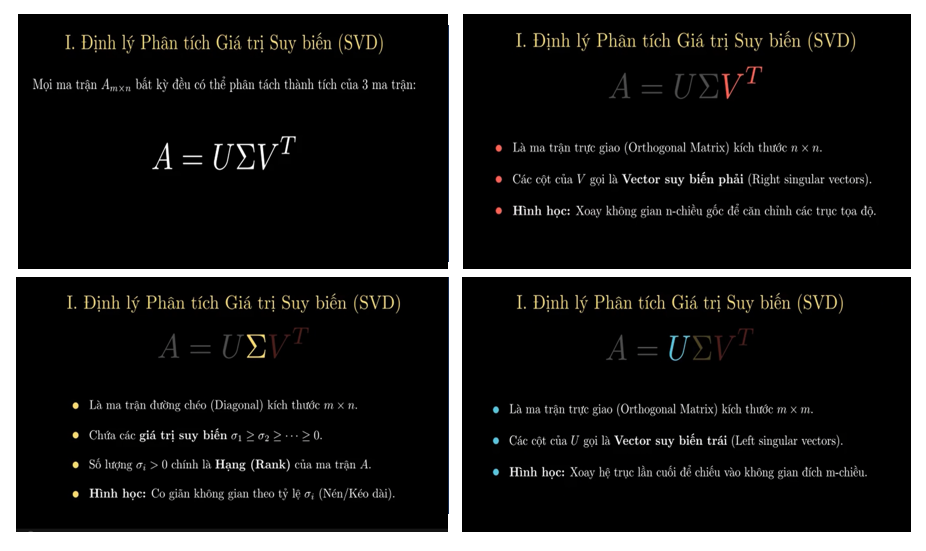
\includegraphics[width=1\textwidth]{images/Ly_thuyet_svd.png}
        \caption{Ảnh minh họa cho phần trình bày lý thuyết SVD.}
        \label{fig:SVD_Lythuyet}
    \end{figure}

    \item \textbf{Mô phỏng trực quan:} Nhóm sử dụng ma trận thực tế $A = \begin{bmatrix} 2 & 1 \\ 1 & 2 \end{bmatrix}$ tác động lên một đường tròn đơn vị và hai vector cơ sở trong không gian 2D. Các hiệu ứng hình học (apply\_matrix) được áp dụng tuần tự theo từng ma trận thành phần, giúp người xem thấy rõ quá trình đường tròn bị xoay, bóp méo thành hình elip và định vị lại.
    
    \begin{figure}[H]
        \centering
        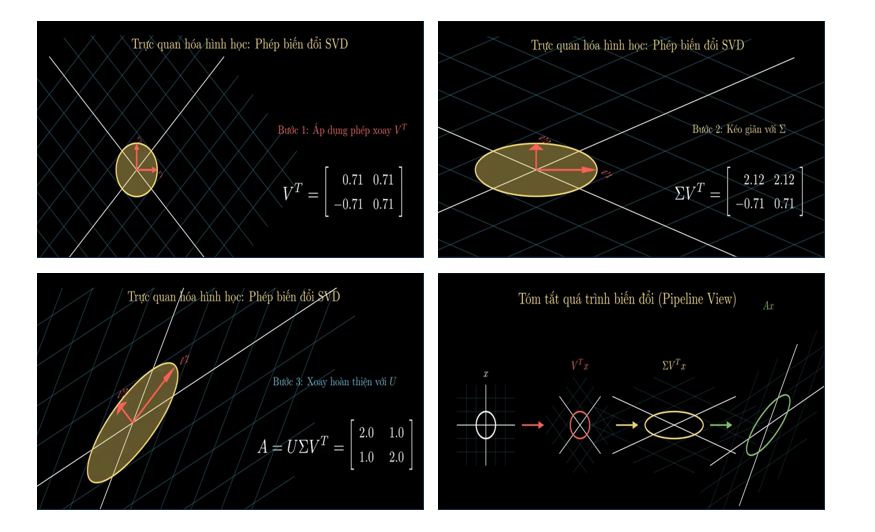
\includegraphics[width=1\textwidth]{images/Truc_quan_svd.png}
        \caption{Mô phỏng trực quan SVD trong không gian 2D.}
        \label{fig:SVD_mo_phong}
    \end{figure}
\end{itemize}

\subsubsection{Trình bày lý thuyết và mô phỏng Chéo hóa ma trận}
\begin{itemize}
    \item \textbf{Mục tiêu:} Trình bày lý thuyết chéo hóa và ứng dụng trong tính toán lũy thừa ma trận.
    \item \textbf{Mô tả kịch bản:} 
    \begin{itemize}
        \item Giới thiệu công thức chéo hóa $A = P D P^{-1}$.
        \item Nhóm lồng ghép hiệu ứng triệt tiêu đại số để làm nổi bật sức mạnh của phép chéo hóa trong việc tính lũy thừa ma trận: $A^n = P D^n P^{-1}$.
    \end{itemize} 
    
    \begin{figure}[H]
        \centering
        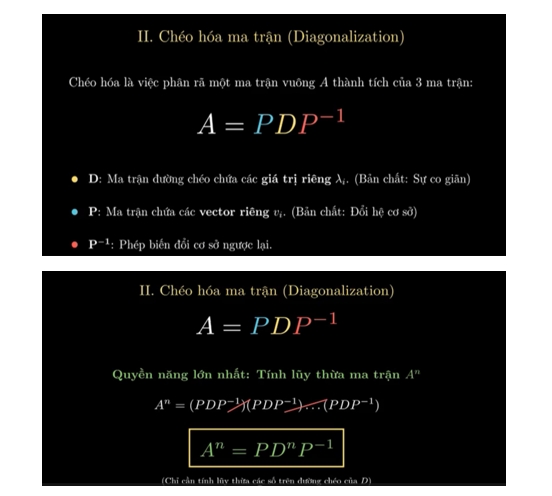
\includegraphics[width=0.75\textwidth]{images/Ly_thuyet_cheo_hoa.png}
        \caption{Ảnh minh họa cho lý thuyết chéo hóa.}
        \label{fig:cheo_hoa}
    \end{figure}

    \item \textbf{Mô phỏng trực quan:} Minh họa từng bước giải bài toán chéo hóa cho ma trận đối xứng. Giao diện video mô phỏng lại quá trình giải phương trình đặc trưng để tìm trị riêng $\lambda$ và vector riêng $v$. Điểm nhấn là hiệu ứng "lắp ráp": các trị riêng di chuyển để tạo thành ma trận đường chéo $D$, trong khi các vector riêng ghép lại thành các cột của ma trận $P$.
    
    \begin{figure}[H]
        \centering
        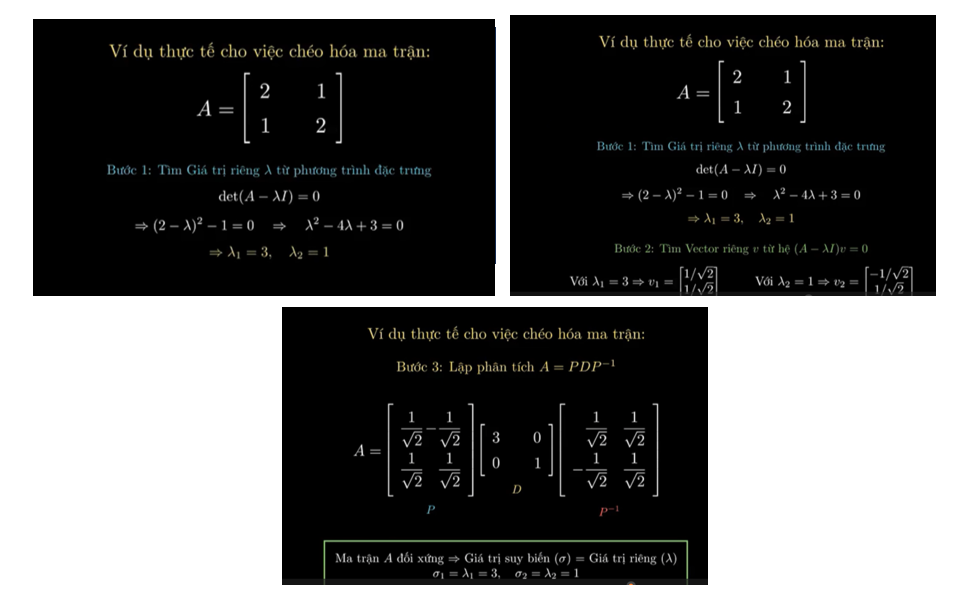
\includegraphics[width=1\textwidth]{images/Truc_quan_cheo_hoa.png}
        \caption{Ví dụ minh họa quá trình lắp ráp ma trận chéo hóa.}
        \label{fig:cheo_hoa_thucnghiem}
    \end{figure}
\end{itemize}

\subsubsection{Mối liên hệ đại số và Ứng dụng nén ảnh}
\begin{itemize}
    \item \textbf{Mục tiêu:} Chứng minh mối liên hệ chặt chẽ giữa hai phương pháp và minh họa tính ứng dụng của SVD trong thực tế.
    
    \begin{figure}[H]
        \centering
        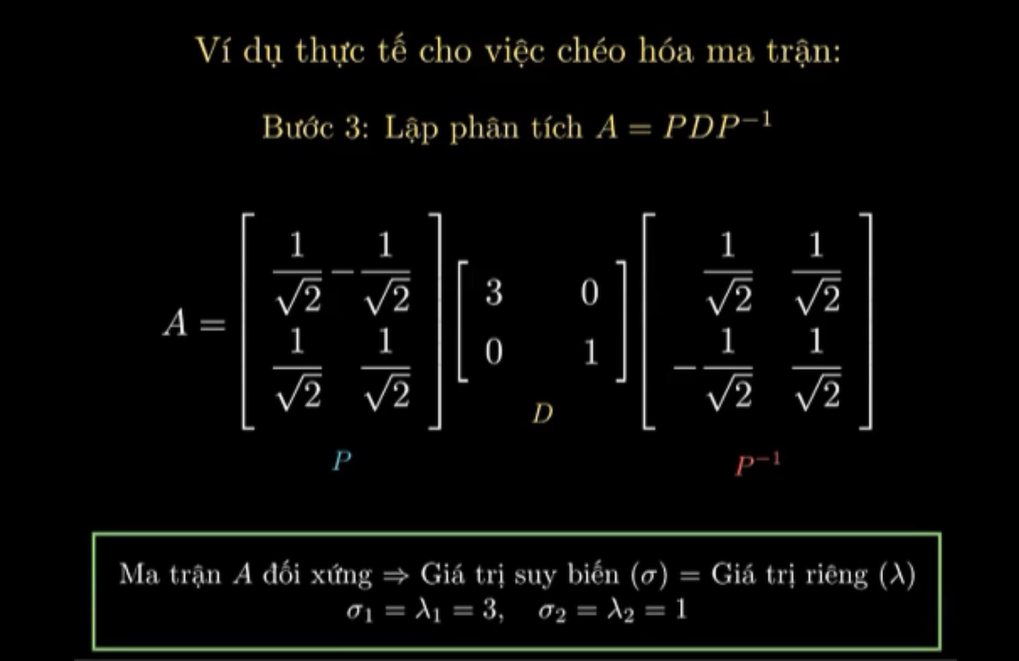
\includegraphics[width=0.75\textwidth]{images/Moi_lien_he.png}
        \caption{Tổng quan mối liên hệ giữa SVD và Chéo hóa.}
        \label{fig:moi_lien_he_svd_cheohoa}
    \end{figure}

    \item \textbf{Chứng minh mối liên hệ:} Kịch bản sử dụng hiệu ứng biến đổi công thức (TransformMatchingTex) để đi từ công thức $A^T A = (U \Sigma V^T)^T (U \Sigma V^T)$. Thông qua việc triệt tiêu ma trận trực giao $U^T U = I$ và đổi $V^T = V^{-1}$, hệ thống suy ra kết quả $A^T A = V \Sigma^2 V^{-1}$. Phân cảnh này đưa ra lời giải thích sắc bén: Phép SVD của ma trận $A$ thực chất chính là phép chéo hóa của ma trận $A^T A$, với trị riêng $\lambda_i$ bằng bình phương của giá trị suy biến $\sigma_i$.
    
    \begin{figure}[H]
        \centering
        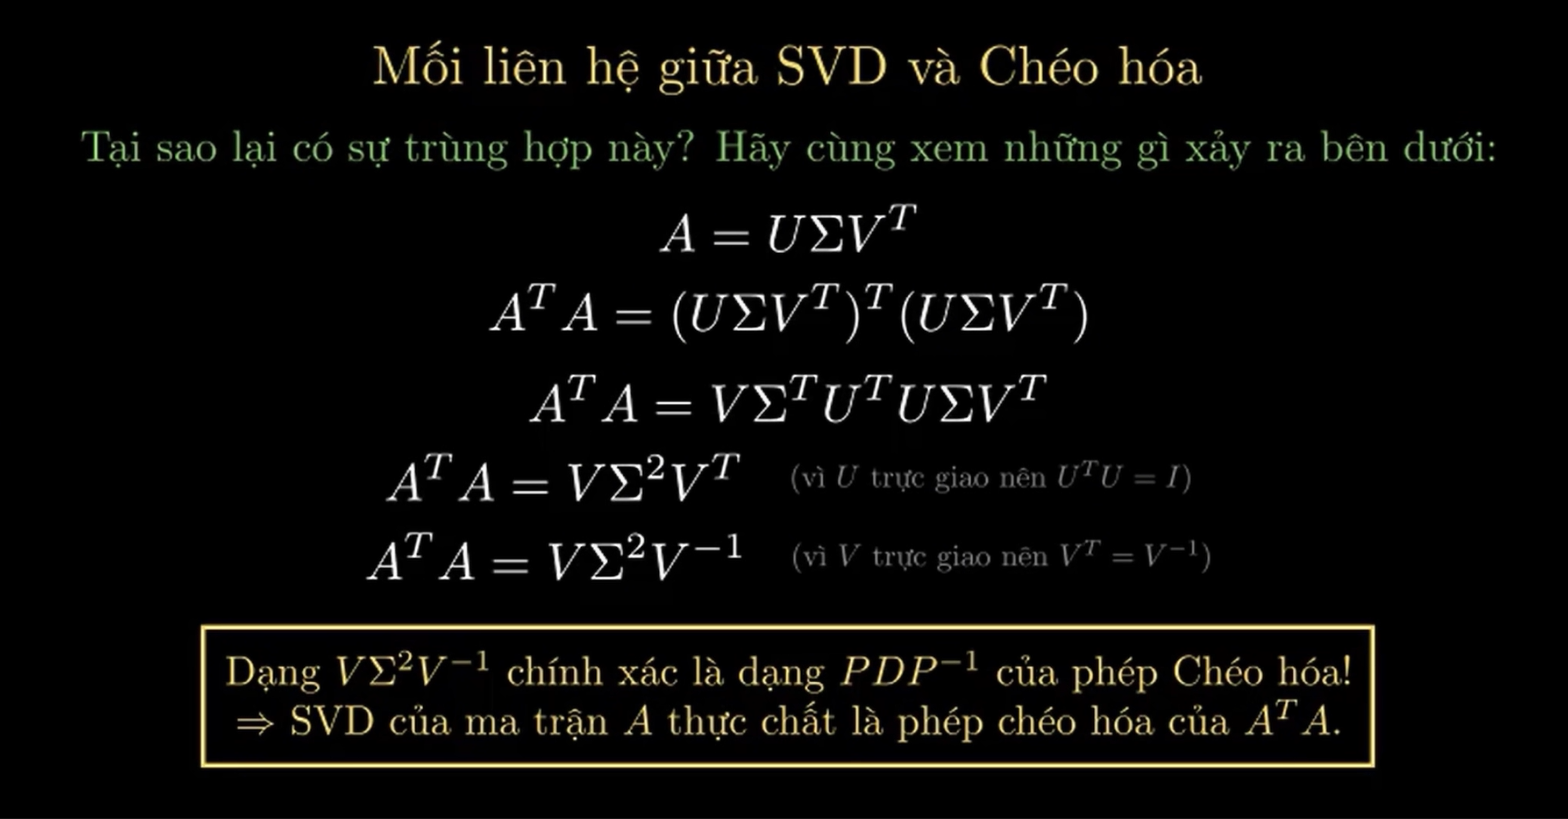
\includegraphics[width=0.75\textwidth]{images/Chung_minh.png}
        \caption{Phân cảnh chứng minh đại số trên Manim.}
        \label{fig:cheo_hoa_va_svd}
    \end{figure}

    \item \textbf{Ứng dụng nén hình ảnh:} Phân cảnh cuối chuyển sang mô phỏng thuật toán SVD rút gọn (Truncated SVD) trên một hình ảnh thực tế (được xem như một ma trận điểm ảnh). Video hiển thị một thanh trượt tham số $k$ (số lượng giá trị suy biến được giữ lại). Khi $k$ tăng dần, bức ảnh từ dạng các mảng mờ nhạt dần trở nên sắc nét, qua đó trực quan hóa khả năng loại bỏ dữ liệu dư thừa và tối ưu hóa không gian lưu trữ của thuật toán SVD.
    
    \begin{figure}[H]
        \centering
        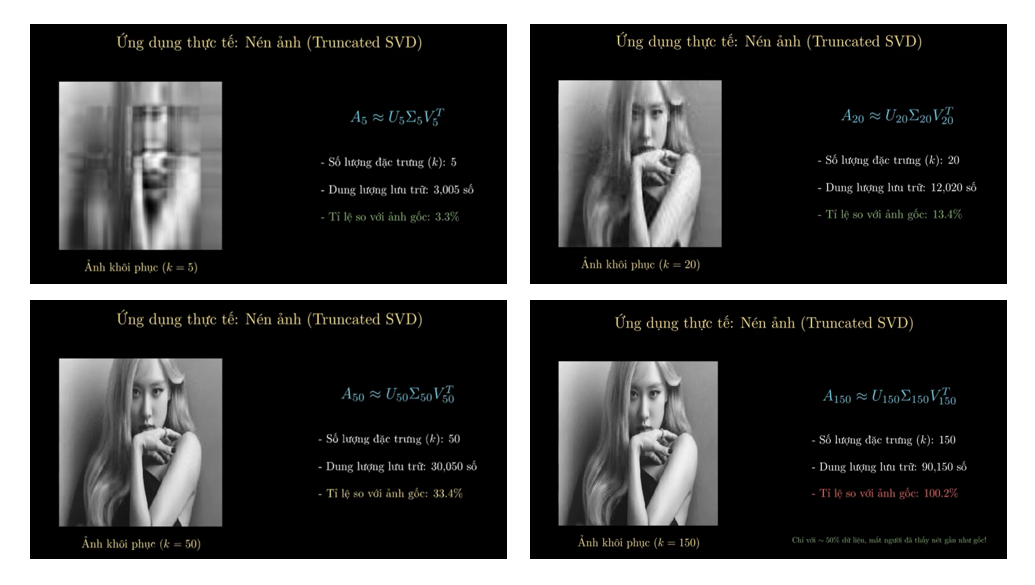
\includegraphics[width=0.8\textwidth]{images/Nen_anh.png}
        \caption{Mô phỏng ứng dụng nén ảnh bằng Truncated SVD.}
        \label{fig:nen_anh}
    \end{figure}
\end{itemize}


\section{Phần 3: Giải Hệ Phương Trình và Phân Tích Hiệu Năng}
\subsection{Cơ sở lý thuyết về sai số và tính ổn định số}
\subsubsection{Chuẩn và Số điều kiện}
Trong tính toán số học, khả năng giải quyết chính xác hệ $Ax=b$ phụ thuộc rất lớn vào số điều kiện $\kappa(A)$. Sử dụng phân rã SVD, ta có:
\begin{equation}
\kappa(A)_2 = \frac{\sigma_{max}}{\sigma_{min}}
\end{equation}
Một bài toán có $\kappa(A)$ lớn được gọi là bài toán "xấu" (ill-conditioned), nơi mà sai số làm tròn có thể phá hủy hoàn toàn ý nghĩa của kết quả tính toán.

\subsubsection{Sai số tương đối}
Để đánh giá kết quả thực nghiệm, chúng tôi sử dụng chuẩn bậc 2 của vector dư (residual vector) chia cho chuẩn của vector vế phải $b$:
\begin{equation}
Error = \frac{\|A\hat{x} - b\|_2}{\|b\|_2}
\end{equation}

\subsubsection{So sánh các phương pháp được thực hiện}
\begin{table}[H]
\centering
\begin{tabular}{|>{\centering\arraybackslash}m{2.5cm}|>{\centering\arraybackslash}m{3cm}|>{\centering\arraybackslash}m{3cm}|>{\centering\arraybackslash}m{3.5cm}|}
\hline
\textbf{Tiêu chí} & \textbf{Khử Gauss} & \textbf{Gauss-Seidel} & \textbf{Phân rã SVD} \\ \hline
\textbf{Độ ổn định} & Trung bình & Phụ thuộc hội tụ & Rất cao \\ \hline
\textbf{Ưu điểm} & Phổ biến, trực tiếp & Tiết kiệm bộ nhớ & Giải được mọi hệ \\ \hline
\textbf{Nhược điểm} & Nhạy với sai số & Khó hội tụ với ma trận xấu & Tính toán phức tạp \\ \hline
\end{tabular}
\caption{Bảng tổng hợp so sánh các phương pháp giải hệ phương trình}
\end{table}

\subsubsection{Phương pháp lặp Gauss-Seidel}
Phương pháp Gauss-Seidel là một thuật toán lặp được sử dụng để giải hệ phương trình tuyến tính $Ax = b$ với $A$ là ma trận vuông cấp $n$. Đây là một cải tiến của phương pháp lặp Jacobi, trong đó các giá trị mới của biến được sử dụng ngay lập tức sau khi chúng được tính toán thay vì đợi đến bước lặp kế tiếp.

\textbf{Cơ sở toán học}

Xét hệ phương trình tuyến tính dưới dạng ma trận $Ax = b$. Ta phân rã ma trận $A$ thành tổng của ba ma trận:
\begin{equation}
    A = D + L + U
\end{equation}
Trong đó:
\begin{itemize}
    \item $D = \text{diag}(a_{11}, a_{22}, \dots, a_{nn})$ là ma trận đường chéo.
    \item $L$ là ma trận tam giác dưới nghiêm ngặt (các phần tử phía trên và trên đường chéo bằng 0).
    \item $U$ là ma trận tam giác trên nghiêm ngặt (các phần tử phía dưới và trên đường chéo bằng 0).
\end{itemize}

Hệ phương trình có thể viết lại dưới dạng:
\begin{align}
    (D + L)x + Ux &= b \\
    (D + L)x &= b - Ux
\end{align}

Từ đó, ta thiết lập công thức truy hồi cho bước lặp thứ $(k+1)$ như sau:
\begin{equation}
    x^{(k+1)} = (D + L)^{-1} (b - Ux^{(k)})
\end{equation}

Dưới dạng khai triển cho từng thành phần $x_i$, công thức lặp Gauss-Seidel được mô tả bởi:
\begin{equation}
    x_i^{(k+1)} = \frac{1}{a_{ii}} \left( b_i - \sum_{j=1}^{i-1} a_{ij} x_j^{(k+1)} - \sum_{j=i+1}^{n} a_{ij} x_j^{(k)} \right), \quad i = 1, 2, \dots, n
\end{equation}

\textbf{Điều kiện hội tụ}

Một điều kiện đủ để phương pháp Gauss-Seidel hội tụ với mọi vector xấp xỉ ban đầu $x^{(0)}$ là ma trận $A$ phải là ma trận \textbf{chéo trội nghiêm ngặt} (Strictly Diagonally Dominant):
\begin{equation}
    |a_{ii}| > \sum_{j \neq i} |a_{ij}|, \quad \forall i = 1, 2, \dots, n
\end{equation}
Ngoài ra, thuật toán cũng hội tụ nếu $A$ là ma trận đối xứng xác định dương (Symmetric Positive Definite - SPD).

\textbf{Tiêu chuẩn dừng}

Quá trình lặp sẽ dừng lại khi nghiệm xấp xỉ đạt được độ chính xác $\epsilon$ cho trước. Tiêu chuẩn dừng thường được xác định dựa trên chuẩn Euclidean của hiệu hai bước lặp liên tiếp hoặc chuẩn của số dư:
\begin{itemize}
    \item Sai số giữa hai bước lặp: $\|x^{(k+1)} - x^{(k)}\|_2 < \epsilon$
    \item Chuẩn số dư: $\|Ax^{(k+1)} - b\|_2 < \epsilon$
\end{itemize}

\subsection{Mô tả thuật toán và cài đặt}

\subsubsection{Các bước thực hiện thuật toán Gauss-Seidel}
\begin{itemize}
    \item \textbf{ Bước 1:} 
    Khởi tạo và thiết lập vector nghiệm ban đầu $x^{(0)} = \mathbf{0}$, ngưỡng sai số $\epsilon$ (tolerance) và số lần lặp tối đa $N_{max}$.
    
    \item \textbf{Bước 2:} 
    Với mỗi bước lặp $k = 0, 1, 2, \dots, N_{max}-1$:
    \begin{itemize}
        \item Lưu trữ nghiệm cũ: $x_{old} = x^{(k)}$.
        \item Cập nhật từng thành phần $x_i$ của vector nghiệm ($i = 1, \dots, n$):
        \begin{equation}
            x_i^{(k+1)} = \frac{1}{a_{ii}} \left( b_i - \sum_{j < i} a_{ij} x_j^{(k+1)} - \sum_{j > i} a_{ij} x_j^{(k)} \right)
        \end{equation}
        \item Kiểm tra tính hợp lệ: Nếu $|a_{ii}| \approx 0$, dừng thuật toán và thông báo lỗi.
    \end{itemize}
    
    \item \textbf{Bước 3:} 
    Kiểm tra hội tụ bằng cách tính chuẩn Euclidean của hiệu hai bước lặp:
    \begin{equation}
        \text{diff} = \sqrt{\sum_{i=1}^{n} (x_i^{(k+1)} - x_i^{(k)})^2}
    \end{equation}
    Nếu $\text{diff} < \epsilon$, thuật toán dừng và trả về nghiệm $x^{(k+1)}$.
    
    \item \textbf{Bước 4:} 
    Nếu đạt đến $N_{max}$ mà không thỏa mãn điều kiện dừng, trả về kết quả hiện tại.
\end{itemize}

\subsubsection{Cài đặt thuật toán Gauss-Seidel}


\begin{lstlisting}[language=Python, caption={Hàm giải thuật toán Gauss-Seidel tách từ solvers.py}]
import math
import part1.matrix as mt
import part1.gaussian_eliminate as ge
import part1.back_substitution as bs
import part2.decomposition as dcp

class Solvers:
    def __init__(self, matrix_obj):
        # Khoi tao voi mot doi tuong Matrix
        self.A = matrix_obj.A
        self.b = matrix_obj.b
        self.n = matrix_obj.n
        self.m = matrix_obj.m
        self.Zero = matrix_obj.Zero

    def solve_gauss_seidel(self, tol=1e-6, max_iter=10000):
        """Giai Ax = b bang phuong phap lap Gauss-Seidel"""
        # Kiem tra ma tran co vuong khong truoc khi thuc hien
        if self.n != self.m:
            raise ValueError("Gauss-Seidel chi ap dung cho ma tran vuong.")
        
        # Khoi tao x la vector 0
        x = [0.0] * self.n
    
        # Kiem tra dieu kien cheo troi chat
        if not self.check_diagonal_dominance(self.A):
            print("Ma tran khong cheo troi — Gauss-Seidel co the khong hoi tu.")

        # Ma tran U la ma tran tam giac tren (khong bao gom duong cheo) chua cac phan tu cua A
        U = []
        for i in range(self.n):
            row = [0.0] * self.n
            for j in range(i + 1, self.n):
                row[j] = self.A[i][j]
            U.append(row)

        for k in range(max_iter):
            # Tao ban sao cua x de so sanh hoi tu
            x_old = x[:] 

            for i in range(self.n):
                # Tinh sum_new: cac phan tu da duoc cap nhat o buoc lap hien tai (j < i)
                sum_new = sum(self.A[i][j] * x[j] for j in range(i))
            
                # Tinh sum_old: cac phan tu tu buoc lap truoc (j > i)
                sum_old = sum(self.A[i][j] * x_old[j] for j in range(i + 1, self.n))
            
                # Cap nhat x[i]
                # Neu tren duong cheo co phan tu bang 0, khong the thuc hien bang phuong phap nay
                if abs(self.A[i][i]) <= self.Zero:
                    raise ValueError(f"Phan tu duong cheo A[{i}][{i}] bang 0.")
                x[i] = (self.b[i] - sum_new - sum_old) / self.A[i][i]

            # Kiem tra dieu kien hoi tu bang chuan Euclidean
            diff_sq_sum = sum((x[i] - x_old[i])**2 for i in range(self.n))
            # Neu khoang cach nay nho hon sai so cho phep, cac gia tri cua x da on dinh
            if math.sqrt(diff_sq_sum) < tol:
                return U, x, k + 1
            
        # Nghiem chua chac da chinh xac, can kiem tra bang phuong phap khac
        return U, x, max_iter
\end{lstlisting}

\subsection{Mô tả quá trình kiểm nghiệm}
% So sánh giữa ma trận Hilbert và SPD ngẫu nhiên
\subsubsection{Phân loại các trường hợp kiểm thử}

\begin{itemize}
\item \textbf{Loại 1 - Ma trận chéo trội nghiêm ngặt (SDD):} Các phần tử đường chéo được thiết lập sao cho $|a_{ii}| > \sum_{j \neq i} |a_{ij}| + \text{rand}(2, 10)$. Đây là điều kiện lý tưởng cho phương pháp Gauss-Seidel.
\item \textbf{Loại 2 - Ma trận chéo trội biên độ lớn:} Tương tự Loại 1 nhưng với biên độ giá trị ngẫu nhiên lớn hơn nhằm kiểm tra độ ổn định số học khi giá trị các phần tử tăng cao.
\item \textbf{Loại 3 - Ma trận không chéo trội (Non-SDD):} Các phần tử đường chéo được cố ý làm nhỏ hơn nhiều so với tổng các phần tử còn lại trên hàng ($|a_{ii}| \approx 0.1 \times \text{off-diag sum}$). Trường hợp này dùng để kiểm chứng sự phân kỳ hoặc lỗi hội tụ của phương pháp lặp.
\end{itemize}

\subsubsection{Các chỉ số đo đạc}

\begin{itemize}
\item \textbf{Thời gian thực thi (Execution Time):} Sử dụng hàm \textbf{time.perf\_counter()} để đo độ trễ tính toán với độ chính xác cao.
\item \textbf{Sai số thực tế (L2 Residual Error):} Được tính theo chuẩn Euclidean của vector dư:
\begin{equation}
\text{Error} = |Ax - b|2 = \sqrt{\sum{i=1}^{n} \left( \sum_{j=1}^{n} a_{ij}x_j - b_i \right)^2}
\end{equation}
\item \textbf{Số bước tính toán (Steps/Iterations):} Đối với phương pháp trực tiếp (Gauss, SVD), số bước mặc định là 1. Đối với Gauss-Seidel, đây là số vòng lặp cần thiết để đạt ngưỡng hội tụ $\epsilon = 10^{-6}$.
\end{itemize}

\subsubsection{Quá trình kiểm thử}

\begin{enumerate}
\item Khởi tạo ma trận $A$ và vector $b$ theo loại và kích thước định trước.
\item Đóng gói dữ liệu vào đối tượng \texttt{Matrix} và khởi tạo lớp \texttt{Solvers}.
\item Gọi lần lượt các hàm:
\begin{itemize}
\item \textbf{solve\_gauss()}: Giải bằng khử Gauss chọn phần tử trụ.
\item \textbf{solve\_svd()}: Giải bằng phân rã giá trị đơn lẻ.
\item \textbf{solve\_gauss\_seidel()}: Giải bằng phương pháp lặp với giới hạn 1000 vòng lặp.
\end{itemize}
\item Tính toán sai số, in báo cáo so sánh kết quả trực tiếp trên màn hình console và lưu dữ liệu vào file Excel.
\end{enumerate}

\textbf{Biểu đồ thời gian chạy, độ hội tụ và log-log: }

\begin{figure}[h]
    \centering
    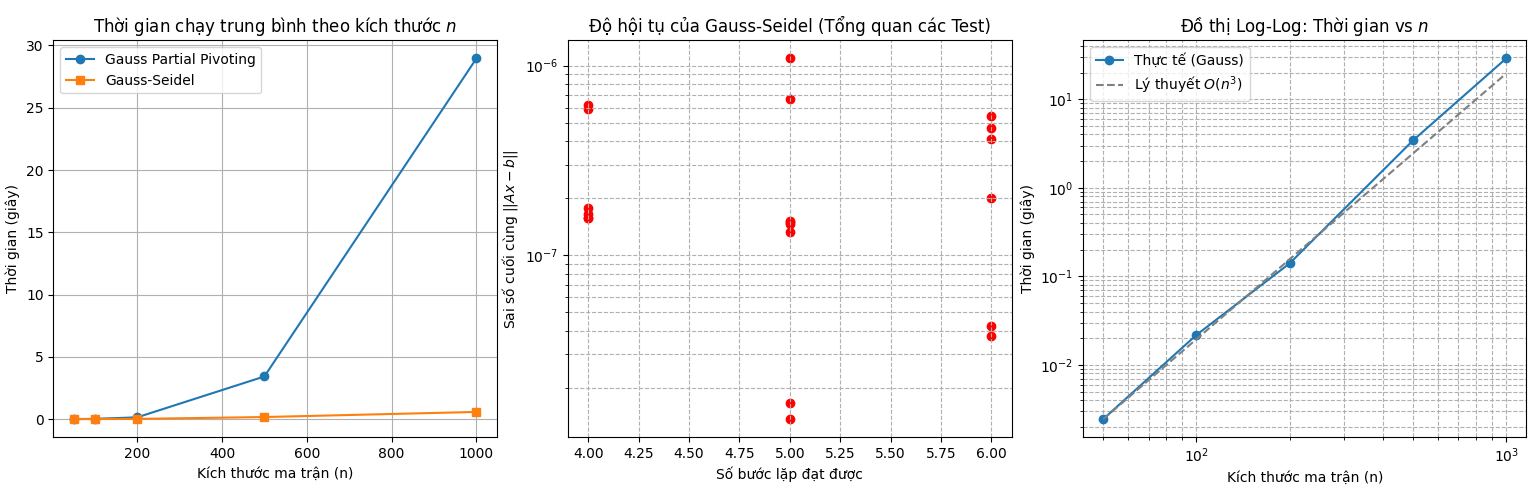
\includegraphics[scale=0.4]{images/test_gauss_seidel_svd.png}
    \caption{Biểu đồ thời gian chạy, độ hội tụ và log-log.}
    \label{fig:my_figure}
\end{figure}


\subsection{Phân tích tính ổn định số}
\subsubsection{Ma trận Hilbert}
\textbf{Định nghĩa: } Ma trận Hilbert là một ma trận vuông mà các phần tử của nó được xác định bởi các đơn phân số. Đây là một ví dụ điển hình trong giải tích số về loại ma trận cực kỳ nhạy cảm với sai số.

Một ma trận Hilbert cấp $n$, ký hiệu là $H_n$, có các phần tử $h_{ij}$ được xác định bởi công thức:
\begin{equation}
    h_{ij} = \frac{1}{i + j - 1}, \quad 1 \le i, j \le n
\end{equation}

Ví dụ, ma trận Hilbert cấp 3 ($H_3$) có dạng:
\begin{equation}
    H_3 = \begin{bmatrix} 
    1 & 1/2 & 1/3 \\ 
    1/2 & 1/3 & 1/4 \\ 
    1/3 & 1/4 & 1/5 
    \end{bmatrix}
\end{equation}

\textbf{Đặc điểm chính:}
\begin{itemize}
    \item $H_n$ luôn là ma trận đối xứng và xác định dương.
    \item Số điều kiện $\kappa(H_n)$ tăng theo hàm mũ $e^{3.5n}$, khiến việc nghịch đảo ma trận này bằng các phương pháp trực tiếp như khử Gauss gặp sai số rất lớn khi $n$ tăng.
\end{itemize}

\subsubsection{Ma trận đối xứng xác định dương (SPD)}
Ma trận SPD (Symmetric Positive Definite) đóng vai trò quan trọng trong các bài toán tối ưu hóa và vật lý kỹ thuật do tính chất hội tụ tốt của các thuật toán liên quan.

\textbf{Định nghĩa:} Một ma trận $A \in \mathbb{R}^{n \times n}$ được gọi là ma trận đối xứng xác định dương nếu thỏa mãn hai điều kiện:
\begin{enumerate}
    \item \textbf{Tính đối xứng:} $A = A^T$.
    \item \textbf{Tính xác định dương:} Với mọi vector $x \in \mathbb{R}^n$ khác không ($x \neq 0$), ta luôn có:
    \begin{equation}
        x^T Ax > 0
    \end{equation}
\end{enumerate}

\textbf{Các tính chất quan trọng:}
\begin{itemize}
    \item Tất cả các trị riêng $\lambda_i$ của ma trận $A$ đều là các số thực dương ($\lambda_i > 0$).
    \item Ma trận $A$ luôn khả nghịch và ma trận nghịch đảo $A^{-1}$ cũng là một ma trận SPD.
    \item Có thể phân rã ma trận $A$ bằng phương pháp Cholesky ($A = LL^T$), đây là phương pháp giải hệ phương trình tuyến tính cực kỳ ổn định về mặt số học.
\end{itemize}

\subsubsection{Mô tả phương pháp ổn định số học}

Để đánh giá độ ổn định số (Numerical Stability) của một ma trận, phương pháp phân rã giá trị suy biến (Singular Value Decomposition - SVD) được sử dụng để tính toán số điều kiện (Condition Number).Số điều kiện của ma trận $A$, ký hiệu là $\kappa(A)$, được xác định thông qua tỷ lệ giữa giá trị suy biến lớn nhất và nhỏ nhất thu được từ phân rã SVD:\begin{equation}\kappa(A) = \frac{\sigma_{\max}}{\sigma_{\min}}\end{equation}

Ma trận Hilbert được chọn làm đại diện tiêu biểu cho nhóm ma trận Ill-conditioned.\begin{itemize}\item \textbf{Đặc điểm trị suy biến:} Kết quả phân tích cho thấy các giá trị suy biến $\sigma_i$ giảm cực kỳ nhanh. Giá trị $\sigma_{\min}$ tiến rất gần về 0 ngay cả khi kích thước ma trận $n$ còn nhỏ.\item \textbf{Số điều kiện:} Do $\sigma_{\min} \to 0$, số điều kiện $\kappa(H_n)$ tăng theo hàm mũ so với $n$. Điều này khiến việc tính toán nghịch đảo hoặc giải hệ phương trình với ma trận Hilbert gặp sai số tích lũy rất lớn.\end{itemize}

\begin{itemize}
\item \textbf{Đặc điểm trị suy biến:} Đồ thị biểu diễn các giá trị suy biến gần như tạo thành một đường nằm ngang. Sự chênh lệch giữa $\sigma_{\max}$ và $\sigma_{\min}$ là không đáng kể.
\item \textbf{Số điều kiện:} Số điều kiện $\kappa$ của ma trận này thường rất nhỏ, dao động quanh mức $1.x$.
\item \textbf{Tính ổn định:} Do $\kappa \approx 1$, thuật toán khi xử lý loại ma trận này sẽ hội tụ nhanh và giữ được độ chính xác cao bất chấp các sai số nhiễu thông thường.
\end{itemize}

\textbf{Kết luận:}

\begin{itemize}
\item Độ tin cậy của một thuật toán (như Gauss-Seidel) không chỉ phụ thuộc vào bản thân phương pháp lặp, mà còn phụ thuộc rất lớn vào đặc tính nội tại (số điều kiện) của ma trận đầu vào.
\item Phân rã SVD là công cụ mạnh mẽ nhất để "chẩn đoán" sức khỏe của một hệ phương trình tuyến tính trước khi tiến hành giải thuật.
\end{itemize}

\textbf{Biểu đồ sự phân bổ giá trị suy biến: }

\begin{figure}[H]
    \centering
    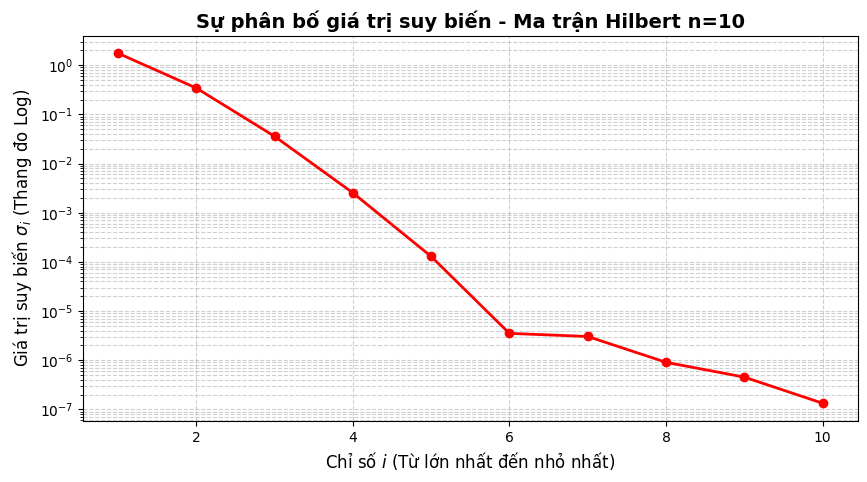
\includegraphics[scale=0.6]{images/hilbert_n10.png}
    \caption{Biểu đồ sự phân bổ giá trị suy biến - Ma trận Hilbert n = 10.}
    \label{fig:my_figure}
\end{figure}

\begin{figure}[H]
    \centering
    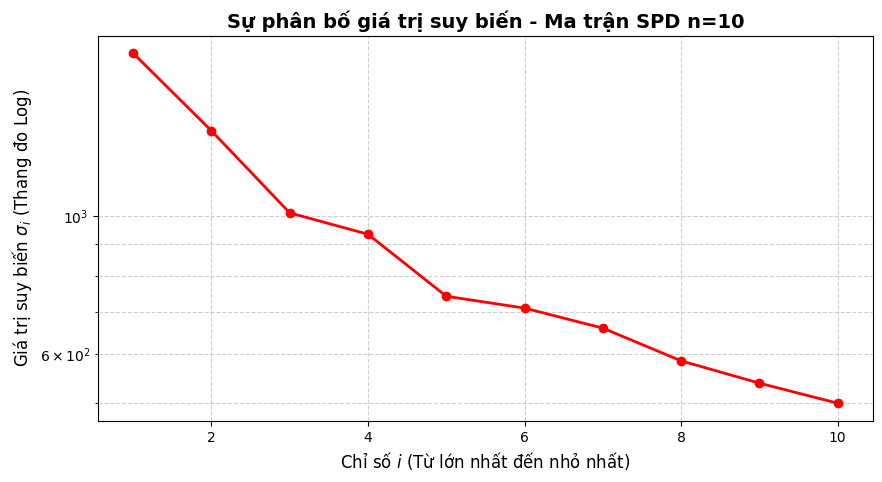
\includegraphics[scale=0.6]{images/spd_n10.png}
    \caption{Biểu đồ sự phân bổ giá trị suy biến - Ma trận SPD n = 10.}
    \label{fig:my_figure}
\end{figure}



\section{Phần 4: Kết luận}
\subsection{Những gì đạt được thông qua đồ án}
Qua quá trình tìm hiểu và cài đặt các thuật toán, nhóm đã có được sự hiểu biết sâu hơn về ma trận và các ứng dụng công nghệ của ma trận vào đời sống
. Cụ thể hơn, nhóm đã làm được những điều sau:
\begin{itemize}
    \item Sử dụng Github để sắp xếp, quản lý dự án.
    \item Rèn luyện khả năng lên ké hoạch và làm việc theo nhóm.
    \item Hiểu được cách giải hệ phương trình bằng ma trận.
    \item Biết cách tái sử dụng và kết hợp các hàm riêng lẻ.
    \item Biết cách kiểm tra và thực nghiệm cho các hàm.
    \item Tìm hiểu, ứng dụng Manim và Latex để xây dựng video học thuật trực quan về toán học.
    \item Phân tích số liệu và vẽ biểu đồ bằng Matplotlib

\end{itemize}

\subsection{Những khó khăn gặp phải}
Việc tìm hiểu của nhóm gặp nhiều khó khăn trong lúc tìm kiếm tài liệu tham khảo và kết hợp các file lại với nhau, nhóm cũng gặp khá nhiều vấn đề trong quá trình kiểm thử và xây dựng video Manim, cụ thể như sau:
\begin{itemize}
    \item Các tài liệu đa số là tiếng Anh khiến việc tiếp thu và áp dụng kiến thức gặp nhiều thiếu sót.
    \item Việc kết hợp các hàm có sai sót trong dữ liệu đầu ra khiến nhóm phải định nghĩa lại dữ liệu đầu ra.
    \item  Trong quá trình kiểm thử, nhóm đã gặp các edge cases với sai số nhỏ, điều đó khiến nhóm phải tái cấu trúc code để đưa ra sai số ít hơn $10^{-9}$. 
    \item Việc mô phòng video Manim gặp khó khăn khi phải tìm animation phù hợp với quá trình mô phỏng phân rã và chéo hoá ma trận.
    \item Thời gian và sai số của các thuật toán khử với từng loại ma trận là khác nhau nên việc đánh giá trường hợp nào sẽ sử dụng thuật khử nào trở nên khó khăn và đa dạng hơn.
\end{itemize}

\subsection{Bài học rút ra}
Thông qua đồ án cùng với những khó khăn mà nhóm gặp phải, nhốm đã đúc kết vả rút ra được các bài học rằng:
\begin{itemize}
    \item Việc lên kế hoạch, định nghĩa cấu trúc code trước khi làm dự án là vô cùng quan trọng.
    \item Phải tìm hiểu từ nhiều tài liệu từ nghiều nguồn khác nhau
    \item  Quản lý code bằng các message khi commit trên github là cần thiết để quản lý tiến trình dự án 
    \item Làm việc nhóm phải có sự liên kết, giao tiếp giữa các thành viên trong nhóm để quá trình làm việc trở nên suông sẻ.
\end{itemize}

\newpage
\begin{thebibliography}{9}
\bibitem{strang2023}
Gilbert Strang. \textit{Introduction to Linear Algebra}, 6th ed. Wellesley-Cambridge Press, 2023.
\bibitem{trefethen1997}
Lloyd N. Trefethen \& David Bau III. \textit{Numerical Linear Algebra}. SIAM, 1997.
\bibitem{geeksforgeeks}
\href{https://www.geeksforgeeks.org/dsa/gaussian-elimination/}{\textbf{Gaussian Elimination to Solve Linear Equations | GeeksforGeeks}}
\bibitem{mit}
\href{https://web.mit.edu/10.001/Web/Course_Notes/GaussElimPivoting.html}{\textbf{Gaussian Elimination with Partial Pivoting (Visualization) | Terry D. Johnson (Massachusetts Institute of Technology)}}
\bibitem{jake@scicoding}
\href{https://scicoding.com/how-to-calculate-matrix-inverse-in-python/}{\textbf{How to Calculate Matrix Inverse in Python | Jake @Scicoding}}
\bibitem{usyd}
\href{https://www.maths.usyd.edu.au/u/geoffp/lm-ss/lectp11.pdf}{\textbf{Column Space Basis | University of Sydney}}
\bibitem{etsu}
\href{https://faculty.etsu.edu/joynerm/documents/RowSpaceColumnSpace.pdf}{\textbf{Row Space, Column Space, and Nullspace | East Tennessee State University}}
\bibitem{googlecolab}
\href{https://www.youtube.com/watch?v=uBY06NpnLcs&t=5s}{\textbf{Post Jupiter Notebooks to a GitHub Repository | Google Colab}}
\bibitem{stanforduniversity}
\href{https://www.youtube.com/watch?v=P5mlg91as1c}{\textbf{Lecture 47 — Singular Value Decomposition | Stanford University}}
\bibitem{machinelearningcoban}
\href{https://machinelearningcoban.com/2017/06/07/svd/}{\textbf{Singular Value Decomposition | Machine learning cơ bản}}

\bibitem{svd_hcmus}
\href{https://machinelearningcoban.com/2017/06/07/svd/}{\textbf{Singular Value Decomposition - Definition and Application}}

\bibitem{jimlambers}
\href{https://web.stanford.edu/class/cme335/lecture7.pdf}{\textbf{Jacobi methods | Stanford University}}
\bibitem{jimlambers}
\href{https://www.geeksforgeeks.org/dsa/matrix-diagonalization/}{\textbf{Matrix Diagonalization | GeeksforGeeks}}
\bibitem{manim}
Manim Community Developers. \textit{Manim — Mathematical Animation Framework}, v0.18. 2024. \url{https://docs.manim.community}
\bibitem{gauss_seidel}
\href{https://www.geeksforgeeks.org/python/gauss-seidel-method/}{\textbf{Gauss Seidel Method | GeeksforGeeks}}
\bibitem{matplotlib}
\href{https://matplotlib.org/}{\textbf{Matplotlib: Visualization with Python}}
\bibitem{matplotlib.pyplot}
\href{https://www.geeksforgeeks.org/python/matplotlib-pyplot-loglog-function-in-python/}{\textbf{Matplotlib.pyplot.loglog() function in Python}}
\bibitem{hilbert_matrix}
\href{https://en.wikipedia.org/wiki/Hilbert_matrix}{\textbf{Hilbert Matrix}}
\bibitem{hilbert_visualization}
\href{https://medium.com/geekculture/visualize-hilbert-matrix-in-python-65955b63b115}{\textbf{Hilbert Matrix Visualization}}

\bibitem{spd_matrix}
\href{https://nhigham.com/2020/07/21/what-is-a-symmetric-positive-definite-matrix/}{\textbf{Definition of SPD Matrix}}

\bibitem{spd_matrix_basics}
\href{https://www.youtube.com/watch?v=cjDf9JdA368}{\textbf{Symmetric Positive Definite Matrix - Basic Theorems}}
\end{thebibliography}

\end{document}

